%-----------------------------------------------------------------------
%                                                                 aa.tex
% AA vers. 9.3, LaTeX class for Astronomy & Astrophysics
% Demonstration file
%                                                       (c) EDP Sciences
%-----------------------------------------------------------------------
%
%\documentclass[referee]{aa}    % for a referee version
%\documentclass[onecolumn]{aa}  % for a paper on 1 column  
%\documentclass[longauth]{aa}   % for long lists of authors and/or affiliations. 
                                % This command displays the first eight authors on page 1
                                % and shift the whole list after the references.
                                % Ensure to separate each author with the \and command (see below)
%\documentclass[letter]{aa}     % for the letters
%\documentclass[bibyear]{aa}    % if the references are not structured
                                % according to the author-year natbib style

\documentclass{aa}

\usepackage{graphicx}
\usepackage{txfonts}
\usepackage{amsmath,amssymb,bm}
\usepackage{subcaption}
\usepackage{lscape}
\usepackage{placeins}
\usepackage{svg}
\usepackage{booktabs}
\usepackage{multirow}
\usepackage{xcolor}
\usepackage[hidelinks]{hyperref}
\usepackage[capitalise,noabbrev]{cleveref}

\renewcommand{\dbltopfraction}{0.9}      % figure* puede ocupar 90% del top
\renewcommand{\dblfloatpagefraction}{0.8}% y 80% de una página de floats
\renewcommand{\topfraction}{0.9}
\renewcommand{\bottomfraction}{0.8}
\renewcommand{\textfraction}{0.07}
\setcounter{dbltopnumber}{2}
\setcounter{totalnumber}{5}

%%% -------- custom macros --------------------------------------------
\newcommand{\Dt}{\Delta t}
\newcommand{\Dm}{\Delta m}
\newcommand{\sDm}[1][]{\sigma_{\Delta m\,#1}}
\newcommand{\madv}{m^{\mathrm{adv}}}
\newcommand{\Dmadv}{\Delta m^{\mathrm{adv}}}
\newcommand{\Lrec}{\mathcal{L}_{\mathrm{rec}}}
\newcommand{\Lmmd}{\mathcal{L}_{\mathrm{mmd}}}
\newcommand{\Lcls}{\mathcal{L}_{\mathrm{cls}}}
\newcommand{\Ltot}{\mathcal{L}_{\mathrm{tot}}}

% Compactar levemente el espaciado alrededor de flotantes (cuerpo a 12 pp)
\setlength{\textfloatsep}{8pt plus 2pt minus 2pt}
\setlength{\intextsep}{8pt plus 2pt minus 2pt}
\setlength{\dbltextfloatsep}{8pt plus 2pt minus 2pt}

% Compactar levemente el espaciado entre referencias (evita pagina casi vacia)
\makeatletter
\renewcommand\@openbib@code{\setlength{\itemsep}{-0.6ex}\setlength{\parsep}{0pt}}
\makeatother

% Permitir a LaTeX empaquetar flotantes de forma mas densa (evita paginas
% con un unico flotante y grandes espacios en blanco)
\setcounter{topnumber}{4}
\setcounter{bottomnumber}{3}
\setcounter{totalnumber}{6}
\renewcommand{\topfraction}{0.92}
\renewcommand{\bottomfraction}{0.85}
\renewcommand{\textfraction}{0.04}
\renewcommand{\floatpagefraction}{0.60}
\renewcommand{\dbltopfraction}{0.92}
\renewcommand{\dblfloatpagefraction}{0.50}

\begin{document}

%%%%%%%%%%%%%%%%%%%%%%%%%%%%%%%%%%%%%%%%
% if you use custom commands in your title,
% ensure to check your title when submitting!
%%%%%%%%%%%%%%%%%%%%%%%%%%%%%%%%%%%%%%%%
\title{Adversarial robustness of variable-star classifiers within the photometric error budget}

\titlerunning{Adversarially robust variable star classifiers}
\authorrunning{C\'aceres et al.}

\author{G.~C\'aceres\inst{1}\fnmsep\thanks{E-mail: gtcaceres@uc.cl}
        \and K.~Pichara\inst{1}
        \and M.~Catelan\inst{2,3}
        \and F.~P\'erez-Galarce\inst{4}
        }

\institute{Computer Science Department, Pontificia Universidad Cat\'olica de Chile
  \and Pontificia Universidad Cat\'olica de Chile, Facultad de F\'isica, Instituto de Astrof\'isica,
       Av. Vicu\~na Mackenna 4860, 7820436 Macul, Santiago, Chile
  \and Centro de Astro-Ingenier\'ia, Pontificia Universidad Cat\'olica de Chile, Av. Vicu\~na Mackenna 4860, 7820436 Macul, Santiago, Chile
  \and Núcleo de Investigación en Data Science, Facultad de Ingenier\'ia y Negocios, Universidad de Las Am\'ericas, Sede Providencia,
       Manuel Montt 948, Santiago, Chile
}

\date{Received \dots; accepted \dots}

% \abstract{}{}{}{}{}
% 5 {} token are mandatory

\abstract
  % context (optional)
  {Machine-learned classifiers reach excellent accuracy in variable-star catalogs, but their stability under perturbations within the reported photometric uncertainties is unknown.}
  % aims (mandatory)
  {We introduce a photometrically bounded threat model in which each magnitude may be displaced only within its reported photometric error interval, quantify the vulnerability of standard light-curve classifiers, and determine what closes this scientific gap.}
  % methods (mandatory)
  {We craft adversarial light curves that shift each observed magnitude only inside its reported error interval, using white-box projected gradient descent and query-only black-box searches. As a defense we train a two-tower convolutional encoder on the raw differential representation $(\Delta t, \Delta m, \sigma_{\Delta m})$ with adversarial training, and audit it with adaptive white-box, gradient-free, margin-based, and attack-potency evaluations on OGLE-III, \textit{Gaia} DR2, and WISE.}
  % results (mandatory)
  {Standard classifiers are vulnerable: a convolutional neural network (CNN) falls from 96.4\% to 65.8\% on OGLE-III, and the $16$-feature random forest loses $6.5$~percentage points (pp) at half the error budget under a feature-recomputing black-box attack. Across surveys, plain adversarial training is the operative defense --- additional consistency, contrastive, and information-bottleneck terms never improve on it --- and the raw differential representation is associated with a further $3$--$7$~pp advantage over an adversarially trained CNN. The defended encoder loses at most $1.0$~pp under adaptive attack ($97.3\%$ on OGLE-III, $90.4\%$ on \textit{Gaia}, $92.5\%$ on WISE, where two under-represented classes limit balanced accuracy to $61.0\%$), and vulnerability scales with the error budget: \textit{Gaia}, with the smallest uncertainties, is nearly immune even undefended. Prediction changes concentrate in $\lesssim 0.5\%$ of sources, providing a per-source robustness flag.}
  % conclusions (optional)
  {Photometric uncertainty defines a physically motivated attack surface, and worst-case-within-errors evaluation is a practical catalog-auditing tool. Adversarial training on a raw differential representation closes the vulnerability at a clean-accuracy cost of ${\sim}0.5$~pp and survives adaptive, gradient-free, and margin-based attacks; the apparent robustness of feature-based methods does not survive attacks tailored to them.}

   \keywords{stars: variables: general -- methods: data analysis -- methods: statistical -- techniques: photometric}

   \maketitle


%%%%%%%%%%%%%%%%%%%%%%%%%%%%%%%%%%%%%%%%%%%%%%%%%%%%%%%%%%%%%%
\section{Introduction}
There have been considerable efforts to automatically classify and extract knowledge from variable star catalogs in recent decades. This focus is primarily motivated by the significance of certain stars (e.g., RR Lyrae and Cepheids), which are critical for measuring cosmological distances \citep{beaton2018distance,bono2024cepheids}. In this context, machine learning models, particularly deep learning approaches, have become crucial in automatically classifying variable stars \citep{aguirre2019deep}. Despite their success, a gap remains in our understanding of the robustness of these models in complex scenarios, such as biased data and low signal-to-noise ratios.

Robustness and uncertainty are closely linked: a robust model must remain stable on noisy or uncertain data. The photometric error is the natural quantification of uncertainty in a light curve, yet while some feature-based classifiers and a few deep models incorporate it as an input or weighting \citep[e.g.,][]{naul2018recurrent}, none has studied the \emph{vulnerability} of the prediction to perturbations contained within it. If a classifier changes its answer under perturbations smaller than the reported measurement uncertainty, its output for that star reflects the particular noise realization that was recorded rather than a property of the star itself.

In this paper, we examine the robustness of these models by assessing their vulnerability to small perturbations constrained by the reported photometric errors. Although these perturbations are bounded by the observational uncertainties, they can significantly alter model predictions, exposing the fragility of standard classifiers. Our contributions are threefold: (i) a photometrically bounded threat model and attack protocol in which every magnitude moves by at most a fixed multiple of its reported uncertainty, together with an auditing methodology (adaptive, gradient-free, and margin-based evaluations, and a per-source robustness flag); (ii) the demonstration, via controlled ablations and an adversarially trained CNN baseline, that standard adversarial training transfers to irregularly sampled light curves at a clean-accuracy cost of only ${\sim}0.5$ percentage points and is the operative defense; and (iii) a robust classifier that combines this training with the raw differential representation of the light curve, which contributes additional clean and adversarial accuracy beyond what adversarial training alone provides.

Worst-case sensitivity is the subject of adversarial-example research: imperceptible input modifications that fool a classifier \citep{goodfellow2014explaining, papernot2016distillation}, and that transfer between models trained on the same task \citep{papernot2016transferability}, enabling benchmark-style robustness comparisons. Adversarial examples are well studied for images but remain underexplored for irregularly sampled time series and no previous work ties the size of the allowed perturbation to the reported uncertainty of each individual measuremment. Figure~\ref{fig:ejemploinicial} shows a light-curve example: the two curves are indistinguishable within their error bars, yet a standard convolutional classifier assigns them to different classes.

Robustness to adversarial examples also carries collateral benefits --- adversarial training can reduce overfitting \citep{miyato2015distributional} and adversarial examples retain class-relevant information useful under imbalance \citep{ilyas2019adversarial} -- and in astronomy, observational effects such as noise or PSF blurring can act as natural adversarial perturbations \citep{ciprijanovic2021robustness}. 

Defense methods either inject adversarial examples into training --- the minimax adversarial training of \citet{madry2017towards}, extended by the clean--adversarial consistency term of \citet{zhang2019theoretically} --- or denoise the inputs with generative models \citep{samangouei2018defense, li2019defense}. These strategies have been developed almost exclusively for images, and their transfer to unevenly sampled astronomical time series has not been tested.

In this paper, we examine the robustness of variable-star classifiers by assessing their vulnerability to small perturbations constrained by the reported photometric errors: every magnitude is allowed to move by at most a fixed multiple of its reported uncertainty. We first demonstrate the vulnerability of traditional classifiers --- Random Forest (RF), convolutional neural network (CNN), and recurrent neural network (RNN) baselines --- on data from the Optical Gravitational Lensing Experiment (OGLE-III; \citealt{udalski2004optical}), \textit{Gaia} Data Release 2 (DR2; \citealt{gaia2018gaia}), and the Wide-field Infrared Survey Explorer (WISE; \citealt{wright2010wide}), and show that the apparent robustness of feature-based classifiers degrades when the attack targets them directly. We then present a supervised classifier that operates directly on the raw differential representation of the light curve --- per-point time differences $\Delta t$, magnitude differences $\Delta m$, and their propagated photometric uncertainties $\sigma_{\Delta m}$ --- and is explicitly trained to be robust to perturbations within the photometric error, and we use controlled ablations to establish which components of the training objective are responsible for that robustness. Finally, we audit the resulting model with adaptive, gradient-free, and margin-based attacks. To our knowledge, this is among the first studies of photometrically bounded adversarial perturbations in variable-star classification operating directly on the observed time series.

This paper is organized as follows. In Sect.~\ref{relatedwork}, we review previous work on variable star classification and adversarial learning. Section~\ref{method} details the proposed model, and Sect.~\ref{datasets} describes the data sets used. Section~\ref{results} presents our results, Sect.~\ref{sec:discussion} discusses their implications and limitations, and Sect.~\ref{conclusion} concludes.
%%%%%%%%%%%%%%%%%%%%%%%%%%%%%%%%%%%%%%%%%%%%%%%%%%%%%%%%%%%%%%

\begin{figure*}
    \centering
    \begin{subfigure}{0.47\linewidth}
        \centering
        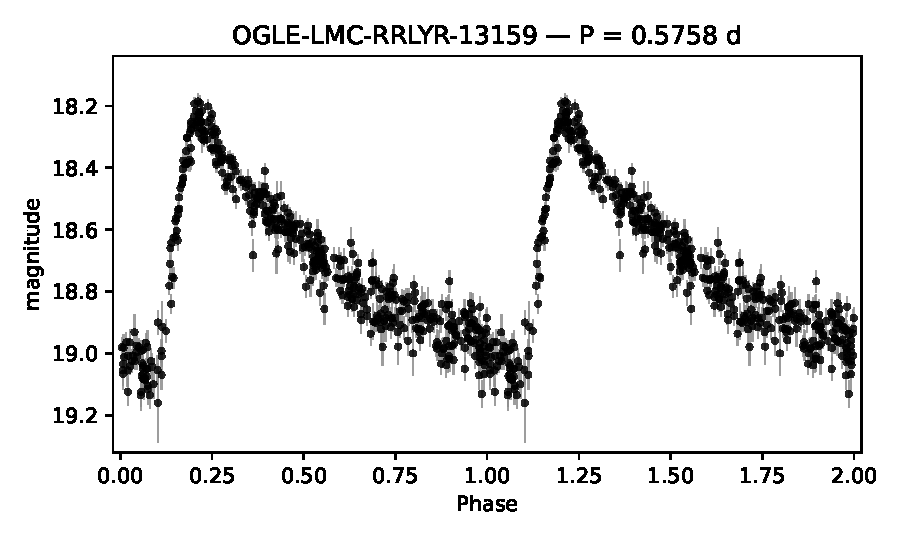
\includegraphics[width=\linewidth]{fig1_clean_errorbars.pdf}
        \caption{Original light curve}
        \label{fig:ejemplo_clean}
    \end{subfigure}
    \hfill
    \begin{subfigure}{0.47\linewidth}
        \centering
        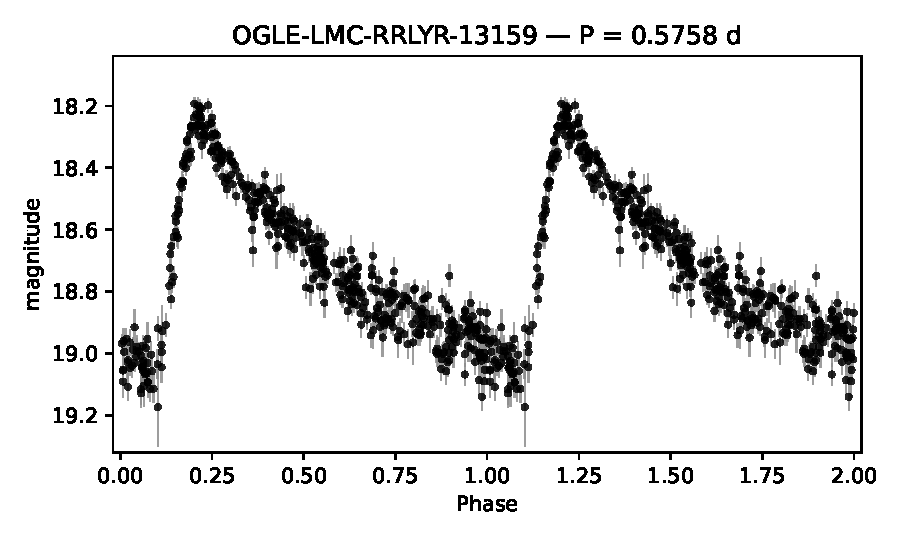
\includegraphics[width=\linewidth]{fig1_adversarial_errorbars.pdf}
        \caption{Adversarial light curve}
        \label{fig:ejemplo_adv}
    \end{subfigure}
    \caption{Original and adversarial versions of the same OGLE RR~Lyrae
    source (OGLE-LMC-RRLYR-13159), phase-folded with its $0.576$-day period
    and shown with the reported per-point photometric uncertainties
    $\pm e_i$ as error bars. Panel (a) shows the clean light curve, and
    panel (b) shows the adversarial version drawn from the adversarial test
    set of Section~\ref{adv_generation}: each observed magnitude is
    displaced within the pointwise bound $|m^{\mathrm{adv}}_i - m_i| \le
    k\,e_i$ at the default budget $k=0.5$. By construction, every displaced
    magnitude remains inside its error interval --- the two panels are
    visually almost indistinguishable --- yet the bounded displacement changes the
    CNN prediction from RR~Lyrae to Cepheid.}
    \label{fig:ejemploinicial}
\end{figure*}
%%%%%%%%%%%%%%%%%%%%%%%%%%%%%%%%%%%%%%%%%%%%%%%%%%%%%%%%%%%%%%

\section{Related work} \label{relatedwork}

\subsection{Variable star classifiers} \label{varstars}

Machine-learned classification of variable stars was first built on
hand-engineered features. \citet{debosscher2007automated} pioneered the
approach with 28 photometric features on OGLE and MACHO data;
\citet{richards2011machine} were the first to incorporate the photometric
error explicitly (through the \texttt{beyond1std} feature), and the FATS
library \citep{nun2015fats} consolidated over 65 features, seven of which
are error-aware. Subsequent work used error-aware features to suppress
spurious variability detections \citep{sokolovsky2017comparative,
pashchenko2018machine} and modeled sparse light curves probabilistically
with Gaussian processes \citep{castro2018uncertain}.

Deep classifiers later replaced feature extraction with end-to-end
learning on the light curve itself, and several explicitly use the
photometric error: the autoencoding RNN of \citet{naul2018recurrent}
weights its loss by the heteroskedastic uncertainties, an idea extended
with Gaussian-mixture modeling by \citet{tsang2019deep};
\citet{hosenie2020imbalance} augment minority classes with Gaussian-process
resampling of the errors; \citet{donoso2021effect} feed the raw triplets of observation time $t$, magnitude $m$, and photometric error $e$
directly to (phased) long short-term memory networks (LSTMs); and \citet{kang2023periodic} scale synthetic
uncertainties to match real ones in an RNN--CNN hybrid. In all of these
works the error improves average accuracy or tolerance to noise; none
evaluates stability under worst-case perturbations within the error bars.

The current state of the art is dominated by transformer-based and
self-supervised representations. \citet{donoso2023astromer} propose ASTROMER, they pre-train a transformer encoder on millions of unlabeled curves, and its successor ASTROMER~2 \citep{donoso2026astromer2} weights the pre-training loss by the reciprocal photometric uncertainties. \citet{cabrera2024atat} combine light-curve and tabular transformers for
alert streams. Contrastive pre-training has also been applied to large
photometric archives \citep{ding2026starclr}, a mechanism related to the
supervised contrastive term of our objective (Sect.~\ref{sec:loss}).
Closest to our concerns, \citet{cadiz2024uncertainty} equipped
ASTROMER-based classifiers with predictive-uncertainty estimates. All of
these models, however, are trained and evaluated on clean inputs. A
complementary line of work addresses reliability under training-set bias
and distribution shift for RR Lyrae classifiers
\citep{perez2021informative, perez2023informative, perez2025self};
that notion of robustness operates at the population level, whereas the
instance-level stability studied here --- the worst-case sensitivity of a
single prediction within the reported error bars --- had not been
evaluated for variable-star classifiers prior to this work.

\subsection{Adversarial learning}
\label{adversarial}

Adversarial examples --- small input perturbations that flip a model's
prediction --- were first demonstrated for deep networks by
\citet{szegedy2013intriguing} and attributed to their locally linear
behavior by \citet{goodfellow2014explaining}. They transfer across
architectures and training sets \citep{papernot2016transferability,
liu2016delving, dong2018boosting}, which enables black-box attacks. For
time series, \citet{fawaz2019adversarial} showed that small perturbations
fool standard deep classifiers for univariate series, and
\citet{karim2020adversarial} extended the result to multivariate series
with a distilled-network attack; the architectures they attack are the
standard CNN/RNN families reviewed by \citet{ismail2019deep}.
\citet{pialla2022smooth, pialla2023time} showed that adding a smoothness
penalty to iterative time-series attacks yields perturbations that are
harder to detect at no cost in effectiveness --- the same attack family
that our smoothness-regularized projected gradient descent PGD (Sect.~\ref{adv_generation}) and its detectability analysis (Appendix~\ref{app:detect}) build on. 

In astronomy, adversarial fragility has been documented in several data modalities:
\citet{gebhard2019convolutional} exhibited adversarial failure modes of
convolutional gravitational-wave detectors; \citet{campagne2020adversarial}
applied adversarial training to photometric-redshift networks;
\citet{ciprijanovic2021robustness} found that observational noise can act
as a natural adversarial example for galaxy-morphology classifiers
trained on simulated images representative of the Legacy Survey
of Space and Time (LSST) at the Vera C. Rubin Observatory \citep{ivezic2019lsst};
\citet{horowitz2022plausible} biased direct parameter-inference networks
with small-amplitude systematics; and \citet{jadhav2023towards} used
adversarial attacks to expose, and then retrain away, failure modes of
gravitational-wave detection models. \citet{bhandari2025interpreting} also examined adversarial robustness in CNN-based classification of gravitational-wave glitches using time--frequency images. For variable-star catalogs, the relevant question is whether predictions remain stable under perturbations of irregularly sampled light curves, with a perturbation budget defined by the reported photometric uncertainty of each observation. None of these works concerns
irregularly sampled photometric time series, and none ties the
perturbation budget to the reported per-point measurement uncertainty, as we do here.

On the defense side, adversarial training \citep{madry2017towards}
remains the standard: the model is trained on worst-case perturbations
within a bounded set. Tradeoff-inspired adversarial defense via surrogate-loss minimization (TRADES; \citealt{zhang2019theoretically}) adds an
explicit consistency term between clean and adversarial predictive
distributions; supervised contrastive learning \citep{khosla2020supervised}
organizes the latent space by class and was extended to adversarial views
by \citet{kim2020adversarial}; and the variational information bottleneck (VIB) \citep{alemi2017deep} limits the input--latent mutual information,
filtering out non-informative perturbations. A complementary, certified alternative is randomized smoothing
\citep{cohen2019certified}, which is natural to mention in this context
because Gaussian measurement noise has a direct physical meaning for
photometric data; we focus on empirical adversarial training and leave
certified defenses to future work. These strategies have been
developed almost exclusively for images; their application to unevenly
sampled astronomical time series --- both attack methodology and defense
design --- remains essentially unexplored and is the gap this paper
addresses.

%%%%%%%%%%%%%%%%%%%%%%%%%%%%%%%%%%%%%%%%%%%%%%%%%%%%%%%%%%%%%%
\section{Method description} \label{method}

The framework comprises two stages. In Stage~1 we generate photometrically bounded adversarial light curves by training a surrogate CNN in a two-channel $(\Delta t, \Delta m)$ representation and applying a PGD attack constrained by the per-point photometric uncertainty. In Stage~2 we build a supervised classifier that operates directly on the raw differential representation of the light curves and is trained adversarially --- with three optional representation-shaping regularizers -- so that its predictions remain stable under the perturbations generated in Stage~1. An overview of the entire pipeline is shown in Fig.~\ref{fig:pipeline} (Appendix~\ref{app:method}).



\subsection{Stage 1: Photometry-constrained adversarial light-curve generation} \label{adversarial_section}

\subsubsection{Surrogate CNN in $(\Delta t, \Delta m)$ space} \label{cnn_classifier}
We first train a CNN following the two-tower design of \citet{aguirre2019deep}. Each light curve is represented by two aligned one-dimensional sequences of length $N$: the time differences $\Delta t = (t_2 - t_1, t_3 - t_2, \ldots)$ and the magnitude differences $\Delta m = (m_2 - m_1, m_3 - m_2, \ldots)$. The CNN processes each channel with shared one-dimensional convolutional blocks, concatenates the resulting feature maps, and outputs class probabilities via a softmax layer. Once trained, the surrogate provides access to the input gradients $\nabla_{\mathbf{x}}\, \mathcal{L}(h_{\mathrm{cnn}}(\mathbf{x}), y)$, where $\mathbf{x}=(\Delta t, \Delta m)$ and $\mathcal{L}$ is the cross-entropy loss. These gradients are the building block of the adversarial attack described next.

\subsubsection{Iterative PGD attack with magnitude-level hard projection} \label{adv_generation}
Our goal is to craft adversarial curves that fool the classifier while remaining \emph{photometrically bounded}, i.e.\ admissible under the pointwise photometric-error constraint: every perturbed magnitude must stay within a fraction of its reported observational uncertainty. Concretely, for an observed light curve $\{(t_i, m_i, e_i)\}_{i=1}^{N}$ with per-observation photometric uncertainties $e_i$, we seek an adversarial counterpart $\{(t_i, m^{\mathrm{adv}}_i, e_i)\}_{i=1}^{N}$ that shares the original observation times $t_i$ and uncertainties $e_i$ and modifies only the magnitudes within the box constraint
\begin{equation}
\label{eq:photobound}
|m^{\mathrm{adv}}_i - m_i| \;\le\; k\,e_i, \qquad i = 1, \ldots, N,
\end{equation}
where $k \geq 0$ is a real-valued, dimensionless budget parameter.
For this threat model, we restrict $k$ to $[0,1]$, using $k=0.5$
by default and $k=1$ for evaluations at the full reported uncertainty. Coordinate-dependent budgets of this kind have precedent in tabular adversarial machine learning, where per-feature perturbation bounds encode feature semantics \citep{ballet2019imperceptible, erdemir2021nonuniform}; here the per-point bound is set by the measurement uncertainty of each observation.

Because the surrogate CNN of Section~\ref{cnn_classifier} consumes first differences rather than raw magnitudes, the attacked tensor must eventually be expressed in $(\Delta t,\Delta m)$ form. We nevertheless parameterize the attack in the same space in which the physical constraint of Eq.~\eqref{eq:photobound} is defined: the per-observation magnitude displacement
$\delta_i = m_i^{\mathrm{adv}} - m_i$. The first observation is kept fixed ($\delta_1=0$), which removes an arbitrary global magnitude offset that would disappear after differencing. We note that, because the budgets are heteroscedastic, this anchoring is not an exact gauge choice: it explores a strict subset of the set defined by Eq.~\eqref{eq:photobound}, since a feasible $\boldsymbol{\delta}$ shifted by $-\delta_1$ need not satisfy every pointwise bound. We verified empirically that the restriction is immaterial: re-running the adaptive white-box attack of Sect.~\ref{sec:adaptive_attack} on OGLE-III with $\delta_1$ free within its own budget $k\,e_1$ leaves the adversarial accuracy of Robust Raw Encoder (RRE) unchanged at $0.973$ (identical to four decimal places), as expected when one observation out of ${\sim}500$ is released. For a candidate displacement vector $\boldsymbol{\delta}$, the magnitude-difference channel evaluated by the CNN is
\begin{equation}
\Delta m_i(\boldsymbol{\delta}) =
\Delta m_i + \delta_i - \delta_{i-1}, \qquad i \ge 2,
\end{equation}
while the cadence channel $\Delta t$ is never modified.

\paragraph{Magnitude-space PGD update.}
At iteration $r$, PGD updates the raw-magnitude displacement and immediately projects it back to the photometric box:
\begin{equation}
\boldsymbol{\delta}^{(r+1)}
\leftarrow
\Pi_{\mathbf{e},k}\!\left[
\boldsymbol{\delta}^{(r)} +
\boldsymbol{\alpha}\odot
\mathrm{sign}\!\left(
\nabla_{\boldsymbol{\delta}}\,
\mathcal{L}\!\left(
h_{\mathrm{cnn}}(\Delta t,\Delta m(\boldsymbol{\delta}^{(r)})), y
\right)
\right)
\right],
\end{equation}
where $\odot$ denotes element-wise multiplication (the Hadamard
product), and $\Pi_{\mathbf{e},k}$ clips each component to
$[-k e_i,+k e_i]$ and keeps $\delta_1=0$. Thus every iterate, and not only
the final adversarial curve, satisfies Eq.~\eqref{eq:photobound}. The
corresponding heteroscedastic uncertainty used as an input channel by the
defended model is the standard propagated error of the first difference,
\begin{equation}
\label{eq:prop_err}
\sigma_{\Delta m_i} = \sqrt{e_i^2 + e_{i-1}^2}.
\end{equation}
The triple $\{(t_i, m_i+\delta_i, e_i)\}_{i=1}^{N}$ is the final adversarial light curve: it shares the times and reported uncertainties of the original observation, and its magnitudes differ from the clean values by at most $k\,e_i$. When this curve is later fed into any classifier that operates on a differenced representation -- including the surrogate CNN and our own robust classifier (Section~\ref{method_l5}) -- the differential sequences are recomputed from these bounded magnitudes and the original observation times, as described in Section~\ref{sec:input_rep}.

\paragraph{Hyperparameters and smoothness regularization.}
We use $k = 0.5$ throughout this work, $T = 20$ PGD iterations, three random restarts, step size $\alpha_i = 0.2\,k\,e_i$, and a uniform random initialization within the photometric box \citep{madry2017towards}. We adopt $k = 0.5$ as the default operating point because it probes vulnerability well inside the admissible set -- each point moves by at most half its reported $1\sigma$ uncertainty -- while the maximal budget considered, $k = 1.0$, reported alongside, saturates the error bars. The inner loop includes a small temporal smoothness penalty $\lambda_{\mathrm{sm}} = 10^{-3}$ on the second discrete differences of $\boldsymbol{\delta}$, following the smooth time-series attack family of \citet{pialla2022smooth}. This term is \emph{not} meant to make the perturbation mimic photometric noise: while the white-noise component of the photometric error is temporally uncorrelated, correlated effects -- red noise, blending, detrending residuals and other systematics of survey photometry -- do produce temporally structured deviations, and a smooth bounded perturbation is in fact the admissible-set member closest to that family; the penalty itself only steers PGD away from high-frequency, low-gradient solutions. The resulting displacements saturate the pointwise budget but are temporally correlated: Appendix~\ref{app:detect} characterizes this structure and shows that order-sensitive statistics (von Neumann ratio, lag-one autocorrelation) expose the attack while amplitude-based statistics do not.

\subsubsection{Transferability across architectures} \label{transfer_prop}
Adversarial examples generated against one classifier often transfer to others trained on the same task \citep{papernot2016transferability}. To investigate this property in our setting, we evaluated RF, CNN, and RNN on the same set of adversarial light curves generated from the surrogate CNN of Section~\ref{cnn_classifier}, allowing a controlled comparison of the robustness of each architecture under a single shared attack.

\subsection{Stage 2: Robust supervised classifier on raw light curves} \label{method_l5}

\subsubsection{Input representation: raw differential sequences} \label{sec:input_rep}

Our classifier consumes the light curves directly in the time domain. For every light curve $\{(t_i, m_i, e_i)\}_{i=1}^{N}$ we build three aligned sequences of consecutive differences: the time gaps $\Delta t_i = t_i - t_{i-1}$, the magnitude differences $\Delta m_i = m_i - m_{i-1}$, and their propagated uncertainties $\sigma_{\Delta m_i} = \sqrt{e_i^2 + e_{i-1}^2}$ (Eq.~\eqref{eq:prop_err}). Differencing makes the representation invariant to the physically uninformative zero-point of the magnitude scale and to the epoch of the first observation, while retaining the local shape and cadence of the variability. It is the only representation our classifier uses.

\paragraph{Fixed-length sequences and padding.} Light curves have a
heterogeneous number of observations. We adopted a fixed length of $L = 500$ points to retain more of the available observations for classification and adversarial evaluation, particularly in OGLE-III. This sequence length also has precedent in the variable-star classifier of \citet{aguirre2019deep}. Curves with more than $L$ epochs are uniformly
subsampled in index along their full time baseline -- preserving the
native ordering and the long-term cadence rather than discarding the
later epochs -- and shorter curves are right-padded. Padded positions
carry a zero raw difference in every channel, which after the global
standardization described next maps to the constant $-\mu/\sigma$ of each
channel; the convolutions are not masked, so these constant tails are
processed like ordinary input. We consider two aspects of unmasked padding: its interaction with the adversarial attack and its potential effect on classification performance. First, the attack cannot act on the padding: the budget encoding marks padded positions as non-perturbable, so all adversarial displacement is confined to real observations. Second, although global average pooling includes the padded tail -- a potential dilution of the signal for short curves, most acute for \textit{Gaia} DR2, whose ${\sim}20$--$30$ epochs occupy $<6\%$ of the tensor -- the effect is not visible empirically, the clean accuracy of RRE on \textit{Gaia} DR2 is flat with curve length ($0.92$ below $15$ epochs, $0.89$--$0.92$ between $15$ and $40$, and $0.91$ above $40$), with no monotonic degradation as the padding fraction grows.

\paragraph{Global per-channel standardization.} Each channel is standardized with a single mean and standard deviation computed once on the training split and reused for the validation and test splits and for the adversarial counterparts. This keeps clean and adversarial inputs on a common, fixed scale and avoids any per-curve quantity that could itself depend on the class.

The encoder receives two input branches (Sect.~\ref{sec:encoder}): a \emph{cadence channel} $\mathbf{x}_t = \Delta t \in \mathbb{R}^{L \times 1}$ and a \emph{magnitude channel} $\mathbf{x}_m = (\Delta m, \sigma_{\Delta m}) \in \mathbb{R}^{L \times 2}$. The uncertainty sub-channel lets the encoder weight noisy points differently from precise ones, and keeps the differential input self-consistent, since the uncertainty of $\Delta m_i$ must include the independent errors of both measurements. The adversarial budget is enforced separately in raw-magnitude space through $e_i$, so $\sigma_{\Delta m}$ is never modified.

\subsubsection{Encoder architecture with variational bottleneck} \label{sec:encoder}

The classifier is built around a two-tower one-dimensional convolutional encoder following the two-channel CNN of \citet{aguirre2019deep} used for the Stage~1 surrogate: one tower for $\mathbf{x}_t$ and one for $\mathbf{x}_m$, fused before a joint convolutional block.

\paragraph{Two-tower convolutional backbone.} Each tower applies two ReLU convolutional blocks (Conv1D $32{\times}7$, then $64{\times}5$ with stride 2); the feature maps are concatenated and processed by two joint blocks ($192{\times}5$, stride 2; $256{\times}3$), followed by global average pooling and a dense layer of width $256$, whose output we denote $\mathbf{h}_\theta(\mathbf{x}) \in \mathbb{R}^{256}$, with $\mathbf{x} = (\mathbf{x}_t, \mathbf{x}_m)$.

\paragraph{Variational bottleneck.} Following the variational autoencoder construction of \citet{kingma2013auto}, two linear heads on $\mathbf{h}_\theta(\mathbf{x})$ parameterize a Gaussian posterior $q_\theta(\mathbf{z} \mid \mathbf{x}) = \mathcal{N}(\boldsymbol{\mu}_\theta(\mathbf{x}), \mathrm{diag}\,\boldsymbol{\sigma}^2_\theta(\mathbf{x}))$ on a $D = 48$ dimensional latent space. During training a latent sample is drawn with the reparameterization trick, $\mathbf{z} = \boldsymbol{\mu}_\theta + \boldsymbol{\sigma}_\theta \odot \boldsymbol{\epsilon}$ with $\boldsymbol{\epsilon} \sim \mathcal{N}(\mathbf{0}, \mathbf{I})$; at inference we use $\mathbf{z} = \boldsymbol{\mu}_\theta(\mathbf{x})$. This is the stochastic encoder of the VIB \citep{alemi2017deep}, whose Kullback--Leibler (KL) term enters the training objective (Sect.~\ref{sec:loss}).

\paragraph{Classifier and projection heads.} The latent vector feeds a \emph{classifier head} $\pi_\phi$ (Dense$(64) \to$ Dropout$(0.2) \to$ Dense$(4) \to$ Softmax), whose output $\mathbf{p} = \pi_\phi(\mathbf{z})$ enters the cross-entropy and TRADES terms and gives the predicted class, and an $\ell_2$-normalized \emph{projection head} $g_\psi$ (Dense$(128) \to$ Dense$(64)$), used only by the contrastive term and discarded after training. All weights are trained end-to-end from scratch.

\subsubsection{Inner adversarial attack during training} \label{sec:inner_attack}

We follow the adversarial-training minimax recipe of \citet{madry2017towards}: at every training step a worst-case counterpart of each clean curve is generated against the current model, and the parameters are updated to minimize the loss on both. The inner maximization is a short PGD attack parameterized, as in Stage~1, in the space where the constraint of Eq.~\eqref{eq:photobound} is defined: the optimization variable is the raw-magnitude displacement $\delta_i = m^{\mathrm{adv}}_i - m_i$, with $\delta_1 = 0$ and
\begin{equation}
\label{eq:inner_eps}
|\delta_i| \;\le\; \epsilon_i \;=\; k\,e_i, \qquad k = 0.5,
\end{equation}

the budget of Stage~1. Starting from $\boldsymbol{\delta}^{(0)} \sim \mathcal{U}(-\boldsymbol{\epsilon}, +\boldsymbol{\epsilon})$, the attack applies $S = 3$ iterations
\begin{equation}
\label{eq:inner_pgd}
\boldsymbol{\delta}^{(s+1)} \;\leftarrow\; \Pi_{\boldsymbol{\epsilon}}\!\left(\boldsymbol{\delta}^{(s)} + \alpha_i \, \mathrm{sign}\,\nabla_{\boldsymbol{\delta}}\, \mathcal{L}_{\mathrm{CE}}\big(\pi_\phi(\boldsymbol{\mu}_\theta(\mathbf{x}'(\boldsymbol{\delta}^{(s)}))),\, y\big)\right),
\end{equation}
with per-point step $\alpha_i = 0.4\,\epsilon_i$, where $\mathbf{x}'(\boldsymbol{\delta})$ is the input whose magnitude channel is recomputed from the displaced magnitudes, $\Delta m^{\mathrm{adv}}_i = \Delta m_i + \delta_i - \delta_{i-1}$, and re-standardized with the clean statistics, and $\Pi_{\boldsymbol{\epsilon}}$ clips each $\delta_i$ to $[-\epsilon_i, +\epsilon_i]$. The cadence channel and $\sigma_{\Delta m}$ are never modified. Because the projection acts on the displacement at every iteration, Eq.~\eqref{eq:photobound} holds by construction throughout training (we also confirmed it empirically), and the adaptive attack of Sect.~\ref{sec:adaptive_attack} uses the same parameterization, so every adversarial input in this paper satisfies it pointwise. The model is run in inference mode during the attack (no batch-normalization updates, no dropout), so that PGD does not pollute the training statistics; the resulting $\mathbf{x}_{\mathrm{adv}} = (\mathbf{x}_t, \mathbf{x}_m^{\mathrm{adv}})$ is then fed back in training mode, and this single adversarial counterpart is shared by all adversarial terms of the objective below.

\subsubsection{Training objective: adversarial training plus representation-shaping regularizers} \label{sec:loss}

Let $\mathbf{z}$ and $\mathbf{z}_{\mathrm{adv}}$ be the encoder means for $\mathbf{x}$ and $\mathbf{x}_{\mathrm{adv}}$, $\mathbf{p}$ and $\mathbf{p}_{\mathrm{adv}}$ the classifier outputs, and $\mathbf{u}$ and $\mathbf{u}_{\mathrm{adv}}$ the ($\ell_2$-normalized) projection-head embeddings. The training loss is
\begin{equation}
\label{eq:loss_total}
\mathcal{L} \;=\; \mathcal{L}_{\mathrm{CE}}^{\mathrm{cl}} \;+\; \lambda_{\mathrm{adv}}\,\mathcal{L}_{\mathrm{CE}}^{\mathrm{adv}} \;+\; \lambda_{\mathrm{tr}}\,\mathcal{L}_{\mathrm{TRADES}} \;+\; \lambda_{\mathrm{sc}}\,\mathcal{L}_{\mathrm{SupCon}} \;+\; \beta\,\mathcal{L}_{\mathrm{VIB}},
\end{equation}
with the following five terms. (i) The clean cross-entropy $\mathcal{L}_{\mathrm{CE}}^{\mathrm{cl}} = -\log p_y$ anchors clean accuracy. (ii) The adversarial cross-entropy $\mathcal{L}_{\mathrm{CE}}^{\mathrm{adv}} = -\log (p_{\mathrm{adv}})_y$ is the adversarial-training term of \citet{madry2017towards}. (iii) The TRADES consistency $\mathcal{L}_{\mathrm{TRADES}} = \mathrm{KL}(\mathbf{p} \,\|\, \mathbf{p}_{\mathrm{adv}})$ penalizes any prediction shift under perturbation \citep{zhang2019theoretically}.
(iv) The supervised adversarial contrastive loss \citep{khosla2020supervised,kim2020adversarial},
\begin{equation}
\mathcal{L}_{\mathrm{SupCon}} \;=\; -\sum_{i \in \mathcal{I}} \frac{1}{|P(i)|}\sum_{p \in P(i)} \log \frac{\exp(\mathbf{u}_i \cdot \mathbf{u}_p / \tau)}{\sum_{a \in A(i)} \exp(\mathbf{u}_i \cdot \mathbf{u}_a / \tau)},
\end{equation}
pulls clean and adversarial views of the same class together; $\mathcal{I}$ indexes the clean and adversarial views of the batch (two per light curve), $A(i)=\mathcal{I}\setminus\{i\}$, $P(i)\subseteq A(i)$ contains the views sharing the anchor's label (including its paired view), and $\tau=0.1$. (v) The VIB term $\mathcal{L}_{\mathrm{VIB}} = \mathrm{KL}(q_\theta(\mathbf{z}\mid\mathbf{x}) \,\|\, \mathcal{N}(\mathbf{0}, \mathbf{I}))$ compresses the latent representation \citep{alemi2017deep}.

Terms (i)--(iii) constitute the defense proper: the minimax recipe of \citet{madry2017towards}, optionally smoothed by TRADES. Terms (iv) and (v) are representation-shaping regularizers motivated by the latent-space analysis of Appendix~\ref{sec:latent_stability}; the ablation of Sect.~\ref{sec:ablation} shows that they leave accuracy and robustness essentially unchanged, so the five-term configuration is a conservative default rather than five individually necessary defenses. The weights are fixed to $\lambda_{\mathrm{adv}} = 1.0$, $\lambda_{\mathrm{tr}} = 2.0$, $\lambda_{\mathrm{sc}} = 0.5$, and $\beta = 5 \times 10^{-4}$ for all three surveys; the projection head receives gradients only from term~(iv).

\subsubsection{Optimization protocol} \label{sec:optim}

The objective is minimized with Adam \citep{kingma2014adam} (initial learning rate $5 \times 10^{-4}$, batch size $256$) for up to $20$ epochs per survey, halving the learning rate when the adversarial validation accuracy plateaus for four epochs and stopping early after eight (restoring the best weights). A separate model is trained per survey; no data are pooled.

\subsection{Implementation and data availability} \label{sec:implementation}

The pipeline is implemented in Python using TensorFlow~2 and Keras for the neural networks, \texttt{scikit-learn} \citep{pedregosa2011scikit} for the RF baseline, and \texttt{astropy.timeseries} \citep{astropy2022} for the Lomb--Scargle periodogram. The period is not required by our classifier, which operates on raw differential sequences, nor by the RF, whose $16$ features are period-independent (Appendix~\ref{app:baselines}); it is used only for catalog-level quality filtering, applied before any model comparison without class-dependent frequency windows, and for phase-folded visualizations. The adversarial light curves for the three surveys, the cached periods, the trained checkpoints, and the scripts reproducing every stage (surrogate training, adversarial generation, input construction, RRE training, and evaluation) are publicly available at \url{https://github.com/gtcaceres1-ui/adversarial-light-curves}.
%%%%%%%%%%%%%%%%%%%%%%%%%%%%%%%%%%%%%%%%%%%%%%%%%%%%%%%%%%%%%%


\section{Datasets} \label{datasets}

We apply our method to three publicly available variable-star surveys with markedly different photometric properties: the optical \emph{Optical Gravitational Lensing Experiment Survey III} the optical OGLE-III \citep{udalski2004optical, udalski2008ogle} and \textit{Gaia} DR2 \citep{gaia2018gaia} surveys, and the mid-infrared WISE survey \citep{wright2010wide}. Together, these three surveys span complementary regimes of cadence, photometric uncertainty, and wavelength coverage, allowing us to assess the proposed defense under a wide range of observational conditions. For the three surveys we use the curated catalogs and light curves assembled by \citet{becker2020scalable}, who compiled them for multi-survey variable-star classification; Table~\ref{tab:survey_classes} reports the native labels and counts of each catalog.

For all three surveys, we restrict the analysis to the four most populated variability classes available in each catalog and apply a per class random subsample (with a maximum of $20\,000$ light curves per class, seed~42) before the train--test split described in Section~\ref{results_setup}. The resulting class counts after the subsample are summarized in Table~\ref{tab:class_balance}.

\subsection{Surveys}

\emph{OGLE-III} \citep{udalski2004optical, udalski2008ogle} monitored the
Galactic bulge, disk, and Magellanic Clouds in the $I$ and $V$ bands over multi-year baselines, producing well-sampled curves; labels follow the OGLE-III Catalog of Variable Stars
\citep{soszynski2008cep, soszynski2009rrlyr, soszynski2009lpv,
poleski2010dsct, graczyk2011ecl}. We use the four most populated classes
-- eclipsing binaries (ECL; aggregating EC, ESD, ED), RR Lyrae (RRLYR;
RRab, RRc), Cepheids (CEP), and long-period variables (LPV; Miras, SRV,
OSARG) -- and adopt OGLE-III as the primary benchmark, as is standard in
automatic variable-star classification \citep{aguirre2019deep,
becker2020scalable, donoso2021effect, bassi2021classification}.

\emph{Gaia DR2}: we use the all-sky classification of high-amplitude
variable sources of \textit{Gaia} Data Release 2 \citep{gaia_mission,
gaia2018gaia, holl2018gaia, rimoldini2019gaia}, with $G$-band light
curves. \textit{Gaia} curves have few observations per source (typically
${\sim}20$--$30$) and small per-point photometric errors, which restricts
the admissible perturbation budget and provides a complementary regime
for the defense. The working classes are RRLYR (RRAB, RRC, RRD, ARRD),
LPV (MIRA\_SR), CEP (classical, Type~II, anomalous), and $\delta$~Scuti /
SX~Phoenicis (DSCT). We adopt DR2 rather than DR3 -- which expands the variability products to $10.5$ million sources with epoch photometry and $12.4$ million classified \citep{eyer2023gaia, rimoldini2023gaia} -- for comparability with the compilation of \citet{becker2020scalable}, on which our preprocessing, labels, and baselines are built; since DR3 uncertainties are typically smaller, DR2 is also the more conservative stress test.

\emph{WISE} \citep{wright2010wide}: we use $W1$-band ($3.4\,\mu$m) light
curves with labels inherited from the OGLE-III nomenclature
\citep{becker2020scalable}, grouped into the same four classes as
\textit{Gaia}. WISE is the noisiest of the three surveys, so the
photometric budget -- and hence the attack surface -- is largest there;
its CEP and DSCT classes are heavily under-represented in the raw catalog
(Table~\ref{tab:class_balance}), which manifests itself in the per-class
results. The native class labels and counts of the three catalogs are
reported in Appendix~\ref{app:surveys}.

\subsection{Summary of class counts after subsampling}

Table~\ref{tab:class_balance} summarizes the per-class counts entering our experiments. WISE is the most skewed (CEP and DSCT contribute fewer than $3{,}000$ curves \emph{combined}), \textit{Gaia} less so, and OGLE is the most balanced of the three. The final per-class train/test counts after the split, together with the per-object epoch distribution of each survey, are listed in Table~\ref{tab:counts} (Appendix~\ref{app:surveys}).



%%%%%%%%%%%%%%%%%%%%%%%%%%%%%%%%%%%%%%%%%%%%%%%%%%%%%%%%%%%%%%

\section{Results} \label{results}

\subsection{Experimental setup and evaluation protocol}
\label{results_setup}

For each survey, the per-class subsample of Sect.~\ref{datasets} is split into training, validation, and test subsets ($70\%$--$10\%$--$20\%$, stratified by class, seed~$42$). The validation subset is used only for early stopping and learning-rate scheduling (Sect.~\ref{sec:optim}); the test subset is never seen during training or model selection. All classifiers share the same split.

The main cross-survey comparison uses three classifiers: an RF on hand-engineered features \citep[FATS;][]{nun2015fats}, the two-tower CNN of Sect.~\ref{cnn_classifier}, and the proposed RRE of Sect.~\ref{method_l5}. A GRU recurrent baseline following \citet{donoso2021effect} is reported only in the model-specific OGLE-III attack sweep. The RF and CNN are trained on the clean training set with the standard cross-entropy; the RRE is trained with the full objective of Eq.~\eqref{eq:loss_total}, generating a fresh adversarial counterpart of every training batch on the fly (Sect.~\ref{sec:inner_attack}).

Robustness is assessed on adversarially perturbed versions of each test set, generated as in Sect.~\ref{adv_generation} with $k = 0.5$, and all classifiers are evaluated on the same pair of clean and adversarial test sets; we verified on every generated set that the perturbations satisfy Eq.~\eqref{eq:photobound} exactly (Appendix~\ref{app:detect}). For each model and survey we report the clean accuracy $\mathrm{acc}_{\mathrm{c}}$, the adversarial accuracy $\mathrm{acc}_{\mathrm{a}}$, and the drop $\mathrm{acc}_{\mathrm{a}} - \mathrm{acc}_{\mathrm{c}}$ in percentage points (pp). Every metric carries a 95\% percentile-bootstrap confidence interval over the test set ($B=2{,}000$); the clean$\to$adversarial drop and the RRE$-$CNN gap are recomputed within each replicate (a \emph{paired} bootstrap), accounting for the correlation between the two estimators. Alongside accuracy we report balanced accuracy and macro-averaged $F_1$, which weight every class equally and expose minority-class behavior that accuracy can mask (Tables~\ref{tab:bootstrap_main} and~\ref{tab:bootstrap_diffs}).

We first quantify the vulnerability of the baselines under attacks tailored to each model (Sect.~\ref{sec:attack_effectiveness}), then evaluate RRE across the three surveys (Sect.~\ref{sec:l5_robustness}), ablate its loss components (Sect.~\ref{sec:ablation}), and test it against a fully adaptive white-box attack as a first-order check against gradient masking (Sect.~\ref{sec:adaptive_attack}; \citealt{athalye2018obfuscated,carlini2019evaluating}). Per-class breakdowns and latent-space evidence are given in Appendices~\ref{sec:per_class} and~\ref{sec:latent_stability}.

\subsection{Effectiveness of the adversarial attack on supervised baselines}
\label{sec:attack_effectiveness}

% Source CSVs:
%   outputs/metrics/{ogle,gaia,wise}/baselines_clean_vs_adv.csv  (CNN-targeted)
%   outputs/metrics/ogle/whitebox_canonical_sweep.csv            (CNN/RNN targeted)
%   outputs/metrics/ogle/rf_fats_square_attack_k0.50.csv         (Square Attack on RF-FATS16)
%   outputs/metrics/ogle/rf_square_attack.csv                    (Square Attack on RF-Dm7)

To motivate the defense presented in the next subsection, we first show that
the photometrically bounded perturbations of Section~\ref{adv_generation} are
an effective stress test for the standard light-curve classifiers used as
baselines. The astronomical constraint is the same throughout: only the
observed magnitudes are displaced, and every proposed light curve must satisfy
the pointwise photometric bound $|m_i^{\rm adv}-m_i|\le k e_i$. The numerical
search used to find such a curve depends on the classifier only for practical
reasons. For the CNN and RNN we use a gradient-based PGD search; for the
Random Forest, whose features are recomputed from the perturbed photometry, we
use the standard query-based Square Attack \citep{andriushchenko2020square}.
Thus all baselines are tested under the same photometric threat model, even
though the optimizer used to find the bounded perturbation differs. We report
the default budget $k = 0.5$ adopted throughout the paper and, additionally,
the full one-reported-error budget $k = 1.0$, corresponding to a
displacement of one full reported uncertainty per point.

\begin{figure}[t]
\centering
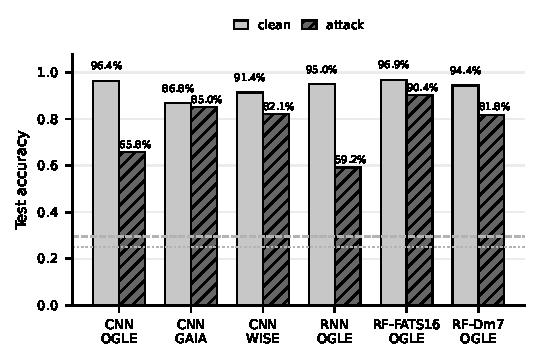
\includegraphics[width=0.86\columnwidth]{baseline_vulnerability.pdf}
\caption{Classification accuracy of the supervised baselines under
photometrically bounded adversarial searches with per-point budget $k = 0.5$.
The CNN is evaluated on all three surveys; the RNN and two RF variants are
shown on OGLE-III. The numerical search is gradient-based for the CNN/RNN and
query-based for the RFs, but every perturbed light curve obeys the same
pointwise photometric bound. Numbers above the bars give the corresponding
test accuracies in percent. The dotted line marks the random-guess level for a
4-class problem; the dashed line marks the majority-class rate of the
OGLE-III test set ($0.29$), the more informative floor for an imbalanced
split. The transferred CNN-targeted cross-survey comparison is
reported separately in Table~\ref{tab:main_multisurvey}.}
\label{fig:baseline_vulnerability}
\end{figure}

\subsubsection{Baseline sensitivity under the same photometric bound}

Under this gradient-based search, the CNN accuracy decreases from $0.964$ to $0.658$ on OGLE-III
($-30.6$~pp) and from $0.914$ to $0.821$ on WISE ($-9.3$~pp), while on
\textit{Gaia} DR2 it only drops from $0.868$ to $0.850$ ($-1.7$~pp): the
small \textit{Gaia} uncertainties shrink the admissible budget $k\,e_i$
itself (Table~\ref{tab:main_multisurvey}). On OGLE-III and WISE the
perturbations push several individual classes below random-guess accuracy
(Appendix~\ref{app:perclass}).

The same gradient-based search is applied to the RNN on OGLE-III, where the
trained instance used for this sweep reaches a clean accuracy of $0.950$.
Under the PGD attack at $k = 0.5$, its accuracy declines to $0.592$
($-35.8$~pp), indicating that the recurrent baseline is also vulnerable to
photometrically bounded perturbations.

For the Random Forest we apply the same photometric logic with a query-based search, since its hand-engineered feature map is not differentiated. We use Square Attack \citep{andriushchenko2020square} on OGLE-III, against two variants. For the actual $16$-feature FATS RF of
Table~\ref{tab:main_multisurvey} (RF-FATS16), every query perturbs the raw magnitudes of the full light curve within the pointwise budget and
recomputes the complete feature vector, so the attack targets exactly the
classifier reported in the main results. On a stratified subsample of
$800$ test curves (clean accuracy $0.969$), the attack reduces the
accuracy to $0.904$ ($95\%$ bootstrap CI $[0.882, 0.924]$; $-6.5$~pp) at
$k = 0.5$ and to $0.805$ ($[0.779, 0.833]$; $-16.4$~pp)
at $k = 1.0$, plateauing after ${\sim}550$ queries. We use a subsample because each query recomputes the full feature vector, which makes the attack computationally expensive; the bootstrap intervals confirm that the accuracy drops are well resolved despite the reduced sample size. A simplified $7$-feature variant in standardized $\Delta m$ space (RF-$\Delta m$7)
falls from $0.944$ to $0.818$ ($-12.6$~pp) at $k=0.5$. Hand-engineered
aggregate statistics therefore confer real but partial protection: the
RF degrades two to five times less than the deep baselines, yet its
apparent immunity under the transferred CNN-targeted perturbations
of Table~\ref{tab:main_multisurvey} does not survive an attack that
targets its own feature space within the same photometric threat model.

\paragraph{Sensitivity to the perturbation budget.}
At the maximal budget considered, $k = 1.0$ (one full reported uncertainty
per point) every baseline degrades monotonically: the CNN falls to $0.465$
($-49.9$~pp), the RNN to $0.427$ ($-52.4$~pp), RF-FATS16 to $0.805$
($-16.4$~pp), and RF-$\Delta m$7 to $0.724$ ($-22.0$~pp); the two neural
baselines approach the four-class random-guess level. Vulnerability to
photometrically bounded perturbations is therefore not a property of any
single architecture --- it affects every supervised classifier evaluated
here, to varying degrees, under gradient-based and query-based attacks.
Table~\ref{tab:targeted_attacks} in Appendix~\ref{app:sweeps} collects these
baseline stress tests at both budgets, and
Fig.~\ref{fig:robustness_vs_k} summarizes them.

\paragraph{A probe of a pre-trained transformer.}
The baselines above are the CNN, GRU, and feature-based classifiers that
have dominated variable-star classification; the current literature is
increasingly moving towards self-supervised transformer representations
(Section~\ref{relatedwork}). As an exploratory probe --- not as a
performance-matched baseline --- we therefore also attacked ASTROMER~2
\citep{donoso2026astromer2}, a transformer foundation model pre-trained
on millions of light curves that, notably, weights its pre-training loss
by the reported photometric uncertainties, making it \emph{a priori} the
most plausible candidate for intrinsic robustness to a photometric attack.
We fine-tuned it end-to-end on the OGLE-III training split following its
published two-phase protocol (frozen-encoder head training, then full
fine-tuning at a low learning rate). It reaches a clean accuracy of
$0.776$ on OGLE-III --- below the from-scratch CNN and RF, which is
expected rather than anomalous: foundation models of this kind are
designed for the few-shot regime \citep{donoso2026astromer2}, whereas our
setup is label-rich (up to $20{,}000$ curves per class), the regime in
which task-specific supervised models are typically strongest. We
therefore do not treat ASTROMER~2 as a state-of-the-art performer on this
task, but as a representative modern architecture. Under the transferred
CNN-targeted attack its accuracy falls to $0.249$ at the maximal budget
$k=1.0$ (drop $-52.6$~pp, $95\%$ bootstrap CI $[-54.0, -51.2]$),
comparable to the collapse of the CNN and RNN in the same setting
(Table~\ref{tab:targeted_attacks}). Even an uncertainty-weighted
transformer representation, then, does not confer robustness within the
photometric budget: the vulnerability documented here is not an artifact
of older architectures.

\begin{figure}[t]
\centering
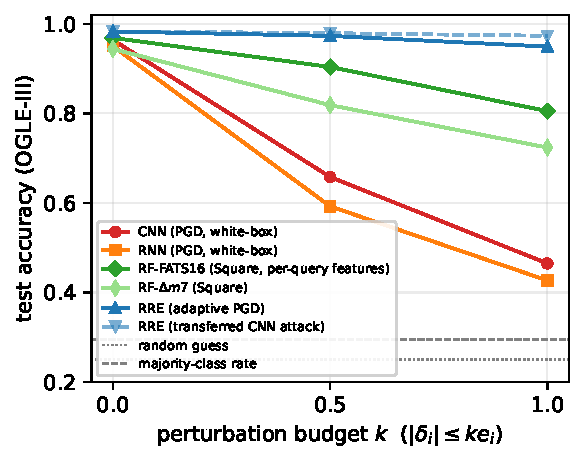
\includegraphics[width=0.86\columnwidth]{robustness_vs_k.pdf}
\caption{Accuracy on OGLE-III as a function of the photometric perturbation
budget $k$ under the same pointwise magnitude bound (solid lines):
gradient-based searches for the CNN and RNN, query-based searches for the RF
variants (RF-FATS16 with per-query feature recomputation), and adaptive PGD
for RRE (at $k=0.5$ and $k=1.0$). The dashed line shows RRE under
the \emph{transferred} CNN-surrogate attack across the full admissible range;
horizontal reference lines mark the four-class random-guess level and the
majority-class rate of the test set.
Adaptive white-box evaluation of RRE on all three surveys is
reported separately in Sect.~\ref{sec:adaptive_attack}.}
% Regenerate with: python3 src/experiments/plot_robustness_vs_k.py
\label{fig:robustness_vs_k}
\end{figure}

% --------------------------------------------------------------------------
\subsection{Robustness of the proposed RRE classifier across surveys}
\label{sec:l5_robustness}

% Source CSVs:
%   outputs/metrics/ogle/robust_raw_eval.csv      (RRE OGLE)
%   outputs/metrics/gaia/robust_raw_eval.csv      (RRE Gaia)
%   outputs/metrics/wise/robust_raw_eval.csv      (RRE WISE)

We now evaluate the Robust Raw Encoder (RRE) of Section~\ref{method_l5}
on the same clean and adversarial test sets used for the baseline
classifiers in Section~\ref{sec:attack_effectiveness}. The model operates
directly on the two-tower $(\Delta t, \Delta m, \sigma)$ representation of
the raw light curve. At inference time, the RRE receives either the clean
or the adversarial counterpart of a given light curve and outputs class
probabilities through its deterministic encoder mean and classifier head
(Section~\ref{sec:encoder}).

Table~\ref{tab:main_multisurvey} compares the clean and adversarial
accuracy of the CNN surrogate, the feature-based RF baseline, and RRE
on the three surveys. The recurrent baseline is kept as an auxiliary
OGLE-only model-specific check in Table~\ref{tab:targeted_attacks}, rather
than as a cross-survey comparator. The RRE preserves its clean accuracy
under the CNN-targeted
attack on all three: the drop is $-0.4$~pp on OGLE-III ($0.983 \to 0.979$),
$-0.5$~pp on \textit{Gaia} DR2 ($0.911 \to 0.906$), and $-0.4$~pp on WISE
($0.932 \to 0.928$).

% Tabla regenerada 2026-06-11 desde outputs/metrics/*/baselines_clean_vs_adv.csv
% y robust_raw_eval.csv (pipeline canónico corregido; ver
% outputs/tables/multisurvey/main_multisurvey.tex).
\begin{table*}
\centering
\caption{Clean and adversarial classification accuracy across the three
surveys under the transferred CNN-targeted attack of
Section~\ref{sec:attack_effectiveness} with $k = 0.5$. Each block of
three columns corresponds to one survey. Two controls isolate the sources of the RRE
robustness: AT-CNN is the \emph{same} surrogate CNN retrained with the
adversarial-training recipe of V2 (isolating the training), and V1 is the
RRE architecture trained with clean cross-entropy only (isolating the
representation). Model-specific adaptive attacks are reported in
Sect.~\ref{sec:ablation}. The RF entries are transfer-attack results, not
robustness certificates: under a model-specific black-box Square Attack
the same OGLE-III RF drops to $0.904$ at $k=0.5$
(Table~\ref{tab:targeted_attacks}). Drop
$= \mathrm{acc}_{\mathrm{a}} - \mathrm{acc}_{\mathrm{c}}$ in pp.}
\label{tab:main_multisurvey}
\begin{tabular}{lrrrrrrrrr}
\toprule
 & \multicolumn{3}{c}{OGLE-III} & \multicolumn{3}{c}{\textit{Gaia} DR2} & \multicolumn{3}{c}{WISE} \\
\cmidrule(lr){2-4}\cmidrule(lr){5-7}\cmidrule(lr){8-10}
Model & $\mathrm{acc}_{\mathrm{c}}$ & $\mathrm{acc}_{\mathrm{a}}$ & drop & $\mathrm{acc}_{\mathrm{c}}$ & $\mathrm{acc}_{\mathrm{a}}$ & drop & $\mathrm{acc}_{\mathrm{c}}$ & $\mathrm{acc}_{\mathrm{a}}$ & drop \\
\midrule
CNN                  & 0.964 & 0.658 & $-30.6$ & 0.868 & 0.850 & $-1.7$ & 0.914 & 0.821 & $-9.3$ \\
AT-CNN               & 0.954 & 0.933 & $-2.1$  & 0.871 & 0.857 & $-1.4$ & 0.916 & 0.903 & $-1.2$ \\
RF                   & 0.976 & 0.925 & $-5.0$  & 0.923 & 0.921 & $-0.2$ & 0.926 & 0.903 & $-2.3$ \\
V1 (clean control)   & 0.988 & 0.916 & $-7.2$  & 0.919 & 0.914 & $-0.5$ & 0.934 & 0.896 & $-3.8$ \\
RRE (ours)           & 0.983 & 0.979 & $-0.4$  & 0.911 & 0.906 & $-0.5$ & 0.932 & 0.928 & $-0.4$ \\
\bottomrule
\end{tabular}
\end{table*}


A paired bootstrap (Appendix~\ref{app:bootstrap}) attaches 95\% confidence intervals to these numbers: the clean$\to$adversarial drop of RRE is $+0.4$, $+0.5$, and $+0.4$~pp on OGLE-III, \textit{Gaia}, and WISE, respectively---each interval excludes zero yet is a small fraction of the corresponding CNN drop---and the adversarial-accuracy advantage of RRE over the CNN ($+32.1$, $+5.6$, and $+10.7$~pp) is significant on all three surveys. The same stability appears in class-balanced metrics: RRE balanced accuracy changes from $97.9$ to $97.5$ on OGLE-III, $88.5$ to $88.0$ on \textit{Gaia} DR2, and $61.0$ to $60.3$ on WISE, while macro-$F_1$ changes from $98.1$ to $97.7$, $89.3$ to $88.7$, and $62.3$ to $61.5$, respectively (Table~\ref{tab:bootstrap_main}).

\paragraph{Survey-by-survey behavior.}
On OGLE-III --- where the attack is most damaging --- the RRE keeps $0.979$ under attack, essentially closing the $30$~pp robustness gap of the CNN. On \textit{Gaia} DR2 the small per-point uncertainties shrink the budget for every model (the CNN drops only $-1.7$~pp). On WISE, the noisiest survey and largest attack surface, the RRE maintains $0.932 \to 0.928$; its aggregate accuracy is driven by the well-represented RRLYR and LPV classes (Section~\ref{sec:per_class_main}), which is why balanced accuracy and macro-$F_1$ are reported throughout.

\paragraph{Reading the clean-accuracy column.}
The clean-accuracy advantage of RRE over the CNN ($+1.9$~pp on OGLE-III) should not be attributed to the defense: the CNN lacks the $\sigma_{\Delta m}$ channel, so the models differ in inputs and training. The architecture-matched clean control is V1, which reaches $0.988$ on OGLE-III --- slightly \emph{above} the defended $0.983$, consistent with the small robustness--accuracy trade-off of Sect.~\ref{sec:ablation}. The informative content of the table is the stability under attack, not the clean ranking.

\paragraph{Does the representation matter, or only the training?}
The AT-CNN row answers this directly: applying the exact adversarial-training
recipe of the V2 variant to the surrogate CNN architecture recovers most
of its robustness (on OGLE-III, from $0.658$ under its own white-box
attack to $0.904$ under an equally aggressive adaptive attack, $T=40$,
five restarts), but it does not close the gap to the raw-representation
models: across the three surveys the AT-CNN remains $3$--$7$~pp below V2
and RRE in both clean and adaptive-attack accuracy (e.g.\ OGLE-III
$0.954$ vs.\ $0.983$ clean, $0.904$ vs.\ $0.973$ adaptive), and it pays
the classical clean-accuracy cost of adversarial training ($-1.0$~pp on
OGLE-III) that the raw encoder largely avoids.
Standard adversarial training is therefore the operative defense, but the raw representation contributes accuracy and robustness that training alone does not supply --- with the caveat that AT-CNN also differs in capacity and lacks the $\sigma_{\Delta m}$ channel, so this is evidence for the representation rather than a controlled attribution. The $3$--$7$~pp gaps are, moreover, well outside the training-seed scatter of the defended variants, which is $0.07$~pp across five seeds on OGLE-III (Section~\ref{sec:ablation}), so single-run comparisons are adequate.

% --------------------------------------------------------------------------
\subsection{Per-class behavior}
\label{sec:per_class_main}

Appendix~\ref{app:perclass} reports per-class accuracies and $F_1$ scores with bootstrap intervals. Robustness is uniform: no class on any survey loses more than ${\sim}2$~pp of accuracy or $F_1$ under the transferred attack, so the aggregate stability of Table~\ref{tab:main_multisurvey} is not an average over heterogeneous behavior. The known limitation is WISE, whose under-represented CEP and DSCT classes (Table~\ref{tab:survey_classes}) are poorly learned or not learned at all on \emph{clean} data by every classifier evaluated here, a clean-trainability effect of catalog imbalance rather than an adversarial vulnerability. We therefore claim no useful absolute performance for WISE CEP and DSCT, for which robustness is vacuous.

\subsection{Ablation study of the V5 loss components}
\label{sec:ablation}

% Source CSV: outputs/metrics/ogle/robust_raw_ablation.csv

To quantify the contribution of each loss component of
Eq.~\eqref{eq:loss_total}, we trained five variants of RRE that add the
terms one at a time: V1 uses clean cross-entropy only (a standard
supervised classifier on the raw two-tower representation); V2 adds
adversarial cross-entropy \citep[Madry-style adversarial
training;][]{madry2017towards}; V3 adds TRADES; V4 adds the supervised
adversarial-contrastive term; and V5 adds the VIB, completing the full
model (the RRE of Table~\ref{tab:main_multisurvey}). Every variant is
trained from scratch on the OGLE-III training split with the same
encoder, optimization protocol (Sect.~\ref{sec:optim}), and inner attack
(Sect.~\ref{sec:inner_attack}); only the loss changes. We evaluate each on
the clean test set, on the same transferred CNN-targeted adversarial set
used throughout the paper, and under the adaptive white-box attack of
Sect.~\ref{sec:adaptive_attack} computed on its own gradient
(Table~\ref{tab:ablation_robust}).

\begin{table}
\centering
\caption{Ablation of the loss components, trained and evaluated directly
on the raw two-tower $(\Delta t, \Delta m, \sigma)$ representation. Top
block: the incremental OGLE-III ladder (each row adds one term to the
previous). Bottom blocks: the V1/V2/V5 comparison repeated on
\textit{Gaia} DR2 and WISE with identical protocols. Transf.\ = transferred CNN-targeted attack;
Adapt.\ = adaptive white-box PGD on each variant's own gradient
(OGLE-III: $T=20$, $3$ restarts; \textit{Gaia}/WISE: $T=40$, $5$
restarts; $k=0.5$). Single runs (seed $42$); five-seed means for V1, V2
and V5 on OGLE-III are in the text (V1: $0.9000 \pm 0.0122$).}
% Fuente: outputs/metrics/{ogle,gaia,wise}/robust_raw_ablation.csv y
% adaptive_pgd_raw_ablation.csv (OGLE 2026-06-12; gaia/wise 2026-07-19).
\label{tab:ablation_robust}
\small
\setlength{\tabcolsep}{4pt}
\begin{tabular}{llrrr}
\toprule
Survey & Variant & $\mathrm{acc}_{\mathrm{c}}$ & Transf. & Adapt. \\
\midrule
\multirow{5}{*}{OGLE-III}
 & V1 (CE only)          & 0.988 & 0.916 & 0.699 \\
 & V2 ($+$ AdvCE)        & 0.984 & 0.979 & 0.971 \\
 & V3 ($+$ TRADES)       & 0.982 & 0.979 & 0.973 \\
 & V4 ($+$ SupCon)       & 0.984 & 0.982 & 0.976 \\
 & V5 ($+$ VIB; full)    & 0.983 & 0.979 & 0.973 \\
\midrule
\multirow{3}{*}{\textit{Gaia} DR2}
 & V1 & 0.919 & 0.914 & 0.912 \\
 & V2 & 0.922 & 0.918 & 0.916 \\
 & V5 & 0.911 & 0.906 & 0.904 \\
\midrule
\multirow{3}{*}{WISE}
 & V1 & 0.934 & 0.896 & 0.840 \\
 & V2 & 0.935 & 0.930 & 0.926 \\
 & V5 & 0.932 & 0.928 & 0.925 \\
\bottomrule
\end{tabular}
\end{table}

The V1 variant, which contains no adversarial component, reaches $0.988$
clean accuracy but loses $7.2$~pp under the transferred attack. This is
already far less than the $30.6$~pp lost by the CNN baseline
(Sect.~\ref{sec:attack_effectiveness}), because the two-tower architecture
and the per-point budget restrict how far the magnitude tower can be
pushed; but the advantage is transfer-specific: under its own adaptive
attack V1 collapses to $0.699$ ($-28.9$~pp), comparable to the CNN under
its own white-box attack ($0.658$). The raw representation on its own is
therefore not robust and, lacking the smoothing that phase binning would
provide, must obtain all of its robustness from the loss.

Adding adversarial cross-entropy (V2) is the dominant step: it lifts the
transferred adversarial accuracy from $0.916$ to $0.979$ ($-7.2 \to
-0.5$~pp) and the adaptive one from $0.699$ to $0.971$, at a clean-accuracy
cost of ${\sim}0.4$~pp ($0.988 \to 0.984$). The accuracy--robustness
trade-off of adversarial training \citep{zhang2019theoretically} is thus
present but small, because the photometric budget is small relative to the
intrinsic variability the encoder must model.

The three remaining
components leave both accuracies essentially unchanged: from V2 to V5 the
clean accuracy stays within $0.2$~pp of $0.984$ and the transferred drop
between $-0.3$ and $-0.5$~pp; under the adaptive attack the latent
regularizers add a small margin ($0.971 \to 0.976$ for V4), partly given
back by the VIB ($0.973$ for V5). These V2--V5 differences of a few tenths
of a point should not be over-interpreted; all four sit far above the
$0.699$ of V1.
\paragraph{The conclusion holds across surveys.}
Because a $0.2$-pp OGLE-III gap could hide a regime where the additional terms matter, we repeated the V1/V2/V5 comparison on the other two surveys (Table~\ref{tab:ablation_robust}, bottom blocks). V2 matches or exceeds V5 on every survey and attack (on \textit{Gaia} it is ${\sim}1$~pp \emph{better}, an order of magnitude above the OGLE-III seed scatter), so no survey provides a regime where the additional terms improve on plain adversarial training. The table also shows that vulnerability scales with the error budget: under its own adaptive attack the undefended V1 loses $28.9$~pp on OGLE-III and $9.4$~pp on WISE, but only $0.8$~pp on \textit{Gaia}, whose tiny uncertainties leave almost no admissible perturbation --- there, the instrument, not the training, is the defense. This is not an artifact of ignoring the faint end, where \textit{Gaia} uncertainties grow \citep[e.g., Fig.~14 of][]{rimoldini2019gaia}: in a random sample of $4{,}000$ of our curves the per-curve median $G$-band uncertainty rises from ${\sim}0.001$~mag at $G < 15$ to ${\sim}0.010$~mag at $G \in [19, 21)$ and $0.015$--$0.027$~mag for the faintest sources ($G \approx 20.7$), still comparable to the $90$th percentile of the OGLE-III budgets ($0.033$~mag) and about half the WISE median ($0.041$~mag), while two thirds of the \textit{Gaia} curves ($G < 18$) sit an order of magnitude below the OGLE-III median ($0.006$~mag).

To quantify the training-seed sensitivity, we repeated the V1, V2, and V5
runs with five independent seeds: the seed-to-seed scatter of the
adversarial accuracy is $0.07$~pp for both V2 ($0.9785 \pm 0.0007$) and V5
($0.9790 \pm 0.0005$), against $1.2$~pp for V1 ($0.9000 \pm 0.0122$), so
adversarial training also stabilizes robustness across runs.
% Fuente multi-seed: outputs/metrics/ogle/multiseed_summary.csv y
% outputs/tables/multiseed_summary.tex (5 seeds: 42,1,2,3,4).
Complementary controls that activate each loss family \emph{without}
adversarial cross-entropy, and a VIB-only $\beta$-sweep, are collected in
Appendix~\ref{app:controls}: TRADES alone matches V2 under the transferred
attack, SupCon alone is only partially robust, and VIB alone is
\emph{not} robust ($-8.0$ to $-9.4$~pp, worsening with compression
strength), corroborating \citet{korshunova2021closer}; random-noise
augmentation is tested in Sect.~\ref{sec:noise_baseline}. We therefore
retain all five components as a conservative full configuration, not as
five individually necessary defenses: AdvCE and TRADES supply the
predictive clean--adversarial coupling, while SupCon and VIB regularize the latent geometry, which Appendix~\ref{sec:latent_stability} shows to be
stable under perturbation, not only at the classifier output.
% --------------------------------------------------------------------------

\subsection{Is random noise augmentation enough?}
\label{sec:noise_baseline}
% Fuente: outputs/metrics/ogle/noise_baseline.csv (2026-06-11).
A perturbation bounded by the photometric error is, by construction,
pointwise compatible with the reported uncertainties, so the most natural
alternative to adversarial training is to augment the training set with
\emph{random} displacements drawn inside the same budget,
$\delta_i \sim \mathcal{U}(-k\,e_i, +k\,e_i)$, or a Gaussian of matching
scale clipped to the same budget, applied with the same raw-magnitude
parameterization as the attack and resampled at every batch. We trained
the V1 encoder (clean cross-entropy only) with each augmentation and
evaluated it under the identical transferred-attack protocol.
Random augmentation provides no measurable protection: the
uniform-noise model reaches $0.987$ clean but $0.914$ adversarial accuracy
($-7.3$~pp), and the Gaussian variant $0.987/0.923$ ($-6.4$~pp) ---
statistically indistinguishable from the un-augmented V1 baseline
($0.9873 \pm 0.0007$ clean, $0.9000 \pm 0.0122$ adversarial across five
seeds; Section~\ref{sec:ablation}), and an order of magnitude worse than
adversarial training ($-0.5$~pp for V2). Exploring the photometric budget
on \emph{average} is therefore not a substitute for optimizing against its
\emph{worst case}: the robustness of RRE is driven by adversarial
training, not by mere exposure to budget-scale input variability.


\subsection{Adaptive white-box attack on the RRE classifier}
\label{sec:adaptive_attack}

% Source CSV: outputs/metrics/ogle/adaptive_pgd_l5_raw.csv

Robustness under a transferred attack can be illusory: defenses must be
evaluated under \emph{adaptive} attacks whose gradient is computed on the
defended classifier itself \citep{carlini2019evaluating}. We therefore
attack the RRE with a white-box PGD back-propagated through its own
encoder and classifier head, using the same raw-magnitude displacement
parameterization as the inner training attack
(Section~\ref{sec:inner_attack}): $\delta_i = m^{\mathrm{adv}}_i - m_i$
clipped to $|\delta_i| \le k\,e_i$ ($k=0.5$) at every iteration, with
$\Delta m$ recomputed by differencing and $\Delta t$ and the uncertainty
channel fixed, so Eq.~\eqref{eq:photobound} holds by construction. The
attack maximizes the true-label cross-entropy far more aggressively than
the training attack: $T = 40$ iterations, per-point step
$\alpha = 0.1\,\epsilon_i$, and $5$ random restarts (keeping the
worst-case restart per curve), versus $S = 3$ single-restart iterations
during training.
% Números regenerados 2026-06-11 con el protocolo descrito (magnitud cruda,
% 40 iter, 5 restarts): outputs/metrics/*/adaptive_pgd_l5_raw.csv.

Under the adaptive PGD attack, the RRE drops from a
clean accuracy of $0.983$ to an adversarial accuracy of $0.973$ on the
OGLE-III test set, a drop of
$-1.0$~pp, against $-0.4$~pp under the transferred attack. The per-class
drops range from $-0.1$~pp on LPV (the largest
and most well-sampled class, $0.998 \to 0.998$) to $-1.8$~pp on ECL
($0.977 \to 0.959$), with RRLYR at $-1.0$~pp and CEP at $-1.3$~pp. Even
this largest
per-class drop is more than an order of magnitude
smaller than the per-class collapses suffered by the CNN baseline
under its own white-box PGD attack
(Section~\ref{sec:attack_effectiveness}).

This conclusion is not specific to OGLE-III. Table~\ref{tab:adaptive_pgd} repeats the adaptive white-box PGD evaluation against RRE's own gradient on all three surveys; the accuracy drop under the adaptive attack does not exceed one percentage point anywhere---$-1.0$~pp on OGLE-III, $-0.7$~pp on \textit{Gaia} and $-0.7$~pp on WISE---so the robustness survives a first-order attack that directly follows the defended model's gradient. This does not certify robustness, but it makes a simple gradient-masking or transfer-artifact explanation unlikely \citep{athalye2018obfuscated,carlini2019evaluating}. At the maximal budget considered ($k=1.0$) the adaptive attack reduces the OGLE-III accuracy to $0.949$ ($-3.4$~pp; Fig.~\ref{fig:robustness_vs_k}).

The adaptive attack is roughly $2.5$ times stronger than the transferred
one ($-1.0$ versus $-0.4$~pp), yet its drop remains more than thirty
times smaller than the CNN's white-box collapse: the robustness of
Section~\ref{sec:l5_robustness} is structural, not an artifact of
gradient transferability. We do not claim certified robustness ---
empirical first-order robustness is the strongest statement an adaptive
PGD evaluation supports.

\subsection{Gradient-free, margin-based, and attack-potency checks}
\label{sec:sanity_checks}
Following the checklist of \citet{carlini2019evaluating}, three further checks (protocols in Appendix~\ref{app:sanity_checks}) complete the evaluation. A gradient-free Square-style attack on the RRE probabilities ($800$ curves, $1{,}000$ iterations, $k=0.5$) costs only $-0.25$~pp, versus $-0.37$~pp for the adaptive white-box PGD run on the same subsample: the gradient-based attack remains the stronger one, the signature of informative, unmasked gradients despite the stochastic bottleneck \citep{korshunova2021closer,athalye2018obfuscated}. The margin-based difference of logits ratio (DLR) loss of Auto-PGD \citep{croce2020reliable} yields $0.973$ at $T=40$ and $T=100$, identical to cross-entropy: the attack is converged and the margin objective finds nothing new. Finally, inflating the budget to $k=5$ and $k=20$ --- far outside the threat model --- collapses the accuracy to $0.135$ and $0.007$: the attack annihilates the model when given room, confirming that robustness at admissible budgets reflects the threat model, not an weak attack.

% --------------------------------------------------------------------------
\section{Discussion}\label{sec:discussion}
The adversarial perturbations considered here are pointwise consistent with
the reported uncertainties: every perturbed magnitude stays within $k\,e_i$
of its observed value, with a fixed budget $k = 0.5$ by default and at most
$k = 1$, so that no measurement is displaced by more than its own reported
$1\sigma$ error. The threat model is therefore bounded by construction. This
bound defines a deterministic uncertainty set rather than a physical hard
limit --- a $1\sigma$ error is the scale of a distribution, not an interval,
and genuine noise exceeds it for roughly a third of the measurements --- so
the perturbations remain well inside the range of displacements that the
reported uncertainties already allow. They are not a stochastic draw from
the survey noise model, but a controlled worst-case stress test: would the
classifier assign the same label to every light curve whose measurements
are pointwise consistent with the reported error bars? If not, the
prediction is sensitive to photometric uncertainty regardless of its
clean-test confidence. Pointwise admissibility is deliberately permissive:
the optimized perturbations are temporally correlated and hence
statistically distinguishable from independent noise
(Appendix~\ref{app:detect}).

This makes the framework a model-auditing tool: photometrically bounded adversarial accuracy complements clean accuracy when validating classifiers, and the clean-to-adversarial prediction change is a per-source \emph{robustness flag} (Table~\ref{tab:flip_rates}; Fig.~\ref{fig:flip_rate}). Under the transferred attack, $30.7\%$, $1.8\%$, and $9.8\%$ of CNN test predictions change on OGLE-III, \textit{Gaia}, and WISE, against $0.4$--$0.5\%$ for RRE. For the defended model the flagged sources are the low-margin ones (median clean margin $0.06$--$0.18$, versus $0.93$--$1.00$ for stable sources), so the flag routes ${\sim}0.5\%$ of sources to follow-up. The undefended CNN shows the opposite, more dangerous pattern: on OGLE-III its flipped sources have a median clean margin of $0.98$, so a confidence cut cannot substitute for the adversarial audit. These flip rates use the true-label attack of the paper; in deployment the same flag is obtained by attacking the clean \emph{predicted} class, or by minimizing the margin $p_1 - p_2$, a label-free variant whose systematic evaluation we leave to future work.

\paragraph{Flagged sources are the noisiest ones.}
The CNN-flagged OGLE-III sources have a median reported error of
$0.053$~mag against $0.007$~mag for the stable ones (a factor of ${\sim}8$;
Mann--Whitney $p \ll 10^{-100}$; Fig.~\ref{fig:flag_quality}) and a lower
per-curve signal-to-noise ratio ($60$ vs.\ $86$). The association is partly
mechanical --- the budget is $k\,e_i$, so noisier sources have more room
to be pushed across the boundary, and the S/N proxy contains $e_i$ --- so
we do not claim it as an independent validation of the flag. It does show
that the flag fires on the noisiest objects rather than on well-measured
ones, the desirable behavior for a follow-up trigger. Testing it against
quality indicators \emph{independent} of $e_i$ (blending or crowding flags,
light-curve-fit $\chi^2$, disagreement with independent classifications)
is a natural next step.

\paragraph{Scope of the threat model.}
The adversarial curves are generated by a surrogate CNN and transferred,
so robustness against the surrogate need not imply robustness against an
attacker with gradient access to RRE itself; we therefore complement the
transferred evaluation with the adaptive white-box attack of
Sect.~\ref{sec:adaptive_attack}. The perturbation set is a per-point box,
$|m_i^{\mathrm{adv}}-m_i|\le k\,e_i$, aligned with the reported
uncertainties; it does not cover structured, $\ell_2$-budgeted, or
time-correlated perturbations, nor perturbations to the sampling times
$t_i$. The robustness we report is also conditional on well-calibrated
uncertainties: under- or over-estimated error bars would shift the
admissible set accordingly. The $k$-sweep of Fig.~\ref{fig:robustness_vs_k}
quantifies this: attacking the $k=0.5$-trained model at $k=1.0$ ---
equivalent to uncertainties underestimated twofold --- lowers the adaptive
OGLE-III accuracy only from $0.973$ to $0.949$. The caveat is most relevant
for WISE: in crowded fields its $W1$ photometry is affected by source
confusion and blending, so the reported per-epoch uncertainties, which do
not fully capture confusion noise, can underestimate the true scatter \citep{cutri2012explanatory,cutri2013explanatory}. Our choice of
\textit{Gaia} DR2 over DR3 (Sect.~\ref{datasets}) is conservative in this
respect: the smaller DR3 uncertainties would shrink the admissible set
further, reinforcing the finding that \textit{Gaia}-like photometry is
nearly immune to the attack. We regard these as boundaries of the present
claims rather than as evidence of unconditional robustness.

\paragraph{Outlook for upcoming surveys.}
The setting becomes operationally relevant with LSST \citep{ivezic2019lsst}, whose alert brokers must classify millions of
variable sources per night from sparse, heteroskedastic photometry.
Worst-case-within-errors evaluation offers such pipelines a training-time
defense costing ${\sim}0.5$~pp of clean accuracy and an offline robustness
audit identifying the ${\sim}0.5\%$ of labels that are not stable within
their own error bars. Because the attack surface scales with the
photometric errors, the audit matters most at the faint end, where the
science is new and the uncertainties are largest.

%%%%%%%%%%%%%%%%%%%%%%%%%%%%%%%%%%%%%%%%%%%%%%%%%%%%%%%%%%%%%%
\section{Conclusions} \label{conclusion}

We studied photometric uncertainty as an attack surface for
machine-learned variable-star classifiers. Adversarial light curves that
displace each magnitude only within its reported error degrade every
standard classifier we evaluated: on OGLE-III the CNN loses $30.6$
percentage points (pp), the GRU $35.8$~pp, and the non-differentiable
$16$-feature RF $6.5$~pp at $k=0.5$ under a query-only black-box Square
Attack; an exploratory probe of a fine-tuned ASTROMER~2 transformer is also
affected. The vulnerability is therefore not an artifact of a particular
architecture, although aggregate feature representations attenuate it
substantially relative to deep sequence models.

As a defense we proposed the Robust Raw Encoder (RRE), a two-tower
convolutional classifier on the raw differential representation $(\Delta
t, \Delta m, \sigma)$, trained adversarially with the per-point photometric
error as the budget of an inner projected-gradient attack. On OGLE-III,
\textit{Gaia} DR2, and WISE it preserves its clean accuracy under attack
(drops of $0.4$--$0.5$~pp, statistically detectable but operationally
negligible; Appendix~\ref{app:bootstrap}), and under an adaptive
white-box attack on its own gradient \citep{carlini2019evaluating} it
loses only $1.0$~pp on OGLE-III, an order of magnitude less than the CNN
under its own attack. The ablation, repeated on all three surveys, shows
that predictive coupling between clean and adversarial views is the
operative ingredient: plain adversarial training (V2) matches or exceeds
the full objective everywhere at a clean-accuracy cost of ${\sim}0.4$~pp,
the remaining terms act as latent-space regularizers, and VIB alone
provides no robustness \citep[corroborating][]{korshunova2021closer}.
Random-noise augmentation within the same budget gives no protection
either, so robustness requires optimizing against the worst case within
the error bars. The representation also matters: an adversarially trained
CNN stays $3$--$7$~pp below the raw-representation models on every
survey. Vulnerability scales with the error budget --- on \textit{Gaia}
even the undefended encoder loses less than one point --- and the defended
model passes the full evaluation checklist (Sect.~\ref{sec:sanity_checks}),
with clean and adversarial views mapped onto the same latent region. Its
main limitation is not adversarial: the under-represented WISE classes are
not learned by any classifier, a catalog property
(Appendix~\ref{app:perclass}).

Future work will extend this
training to further architectures, surveys, and threat models. A natural next step is multiband classification
\citep[e.g.][]{cabrera2024atat}, where the box constraint becomes per band,
$|m^{\mathrm{adv}}_{i,b}-m_{i,b}|\le k\,e_{i,b}$, and a new question
arises: whether perturbations must preserve cross-band (colour) coherence,
a physically motivated restriction with no single-band analogue. The audit
itself is also amenable to automation: an agentic pipeline could
orchestrate gradient- and query-based attacks across budgets and survey
releases, while language models could propose structured, physically
motivated perturbation families (zero-point drifts, seeing- or
blending-dependent systematics) beyond the per-point box, to be then
optimized by the bounded search presented here.

%%%%%%%%%%%%%%%%%%%%%%%%%%%%%%%%%%%%%%%%%%%%%%%%%%%%%%%%%%%%%%


\begin{acknowledgements}
Support for M.C. is provided by ANID’s FONDECYT Regular grant \#1231637 and ANID’s Basal project FB210003. 
We thank the OGLE team for making their photometric database publicly
available. This work has made use of data from the European Space Agency
(ESA) mission \textit{Gaia}
(\url{https://www.cosmos.esa.int/gaia}), processed by the \textit{Gaia}
Data Processing and Analysis Consortium (DPAC,
\url{https://www.cosmos.esa.int/web/gaia/dpac/consortium}). Funding for
the DPAC has been provided by national institutions, in particular the
institutions participating in the \textit{Gaia} Multilateral Agreement.
This publication also makes use of data products from the Wide-field
Infrared Survey Explorer (WISE), which is a joint project of the
University of California, Los Angeles, and the Jet Propulsion
Laboratory/California Institute of Technology, funded by the National
Aeronautics and Space Administration.
\end{acknowledgements}

\section*{Data availability}
The full analysis pipeline and the scripts that reproduce every experiment
are publicly available at
\url{https://github.com/gtcaceres1-ui/adversarial-light-curves}. The
derived data products --- the generated adversarial light curves for the
three surveys, the cached Lomb--Scargle periods used by the Random Forest
baseline, and the trained model checkpoints --- are archived in a Zenodo
deposit (DOI: \texttt{10.5281/zenodo.XXXXXXX}).
% TODO: crear el depósito Zenodo y reemplazar XXXXXXX antes de someter.
The underlying light curves are available from the public OGLE-III,
\textit{Gaia} DR2, and WISE archives, as compiled by \citet{becker2020scalable}.

\bibliographystyle{aa}
\bibliography{bibfile}

% ========================================================
\appendix

\section{Structure, detectability, and budget validation of the perturbations}
\label{app:detect}
\label{sec:pert_struct}
% Empirics: src/experiments/characterize_perturbations.py and
% src/experiments/detectability_features.py; data in
% outputs/perturbation_stats/ and outputs/detectability/.
We measured the temporal structure of the perturbations performed $\boldsymbol{\delta} = \mathbf{m}^{\mathrm{adv}} - \mathbf{m}$ directly on the attacked test sets. At the full perturbation fraction the lag-one autocorrelation of $\boldsymbol{\delta}$ has a median of $0.77$--$0.86$ across surrogates (a null within-curve permutation gives $-0.005$), $96$--$99\%$ of adjacent perturbed points share the same sign (white noise: $50\%$), and the normalized curvature $\sum_i (\Delta^2\delta_i)^2 / \sum_i \delta_i^2$ is suppressed by a factor of $5$--$10$ relative to the shuffled null. Removing the smoothness term does not remove the structure entirely; for the \textit{Gaia} attack ($\lambda_{\mathrm{sm}}=0$) the median autocorrelation lag-one is still $0.26$ --- indicating that the classifier gradients are themselves temporally correlated, with $\lambda_{\mathrm{sm}}$ amplifying the effect. At the same time, the perturbations exhaust the photometric budget pointwise: the median of $|\delta_i| / (k e_i)$ is $1.0$, with $93$--$98\%$ of perturbed points saturating the bound.

This combination --- pointwise admissible amplitudes with non-noise-like temporal ordering --- determines how the attack can and cannot be detected (Table~\ref{tab:detectability}). The distributions of scale-sensitive features in the test set (standard deviation, robust amplitude, Stetson~$K$) are statistically indistinguishable between clean and attacked curves (two-sample KS $D \le 0.022$, $p > 0.08$), so that a survey pipeline monitoring amplitude-like statistics would not notice the attack. Order-sensitive statistics, in contrast, expose it decisively: the attack shifts the von Neumann ratio $\eta_{\mathrm{vN}}$ (median $1.81 \rightarrow 1.64$) and the lag-one autocorrelation of the magnitude sequence (median $0.09 \rightarrow 0.17$), yielding KS statistics of $0.07$--$0.10$ with $p$-values between $10^{-13}$ and $10^{-25}$ at full perturbation fraction, consistently across the OGLE attacks shown below, with a monotonic dose--response as the perturbation fraction grows. For the \textit{Gaia} configuration ($k=0.5$) no feature is significantly displaced, showing that detectability also scales with the budget. These measurements sharpen the sense in which the attack is pointwise admissible --- each magnitude stays within its error bar --- while motivating a cheap audit: flagging curves whose $\eta_{\mathrm{vN}}$ or autocorrelation is anomalous for their class provides a first-line \emph{robustness flag} against smooth bounded attacks, which we return to in the Discussion.

\begin{table*}[htbp]
\caption{Detectability of bounded adversarial perturbations at full perturbation fraction ($f=1.0$): two-sample KS statistic ($p$-value in parentheses) between the clean-test and adversarial-test distributions of standard variability features. The OGLE attacks use $k=1$; the \textit{Gaia} attack uses $k=0.5$. Scale-sensitive features (magnitude scatter $\sigma$, robust amplitude, Stetson $K$) do not separate the two samples, while order-sensitive statistics (von Neumann ratio $\eta_{\mathrm{vN}}$, lag-one autocorrelation ACF$_1$) detect the attack at high significance.}
\label{tab:detectability}
\centering
\small
\begin{tabular}{llccccc}
\hline\hline
Survey & Surrogate & $\sigma$ & Amp. & $K$ & $\eta_{\rm vN}$ & ACF$_1$ \\
\hline
OGLE & CNN & 0.020 (0.15) & 0.022 (0.09) & 0.019 (0.22) & 0.092 ($10^{-23}$) & 0.092 ($10^{-23}$) \\
OGLE & RNN & 0.017 (0.34) & 0.018 (0.26) & 0.018 (0.24) & 0.093 ($10^{-24}$) & 0.095 ($10^{-25}$) \\
OGLE & RF surrogate & 0.017 (0.33) & 0.019 (0.19) & 0.021 (0.14) & 0.071 ($10^{-14}$) & 0.071 ($10^{-14}$) \\
\textit{Gaia} & CNN & 0.019 (1.00) & 0.013 (1.00) & 0.019 (1.00) & 0.013 (1.00) & 0.013 (1.00) \\
\hline
\end{tabular}
\end{table*}


\subsection{Budget validation on the generated test sets}
\label{sec:val_perturb}

% Source CSV: outputs/metrics/ogle/perturbation_validity.csv,
%             outputs/metrics/perturbation_bounds.csv

Before evaluating classifier robustness, we verify empirically that the
adversarial perturbations satisfy the photometric-error budget of
Eq.~\eqref{eq:photobound}. For every observation $i$ in the adversarial test
set of a given survey, we compute the normalized magnitude displacement
\begin{equation}
\delta_i \;=\; \frac{m^{\mathrm{adv}}_i - m_i}{e_i},
\end{equation}
which expresses the change of magnitude in units of the reported photometric
uncertainty. The hard projection step of Section~\ref{adv_generation}
enforces $|\delta_i| \le k$ at every point by construction, and we use the
empirical distribution of $|\delta_i|$ as a diagnostic of the actual
perturbation strength reached by the PGD attack in each survey.

Table~\ref{tab:perturbation_summary} reports summary statistics of
$|\delta_i|$ for the three surveys, computed over all observations of all
light curves in the adversarial test sets. No observation violates the bound
$k = 0.5$ in any of the surveys, as expected from the projection step. The
fact that the median, the 95th percentile and the maximum of $|\delta_i|$
all reach the bound shows that the attack saturates the budget at well over
half of the observations rather than producing trivially small
perturbations. The mean ratio $|\delta_i|/k$ ranges from $0.91$ in
OGLE-III to $0.96$ in \textit{Gaia}, confirming that the attacks use most of
the available pointwise budget while remaining inside the photometric box.

\begin{table}[htbp]
\centering
\caption{Summary of the normalized adversarial displacement
$|\delta_i| = |m^{\mathrm{adv}}_i - m_i|/e_i$ for the three surveys,
aggregated over all observations of all light curves in the corresponding
adversarial test set. The bound $k = 0.5$ is the per-point photometric-error
budget defined in Section~\ref{adv_generation}; no observation violates it
in any of the surveys.}
\label{tab:perturbation_summary}
\setlength{\tabcolsep}{4pt}
\small
\begin{tabular}{lrcccc}
\hline
       &                    & \multicolumn{4}{c}{$|\delta_i|$} \\
\cline{3-6}
Survey & $n_{\mathrm{obs}}$ & Mean & Median & P95 & Max \\
\hline
OGLE-III          &  6{,}281{,}886 & 0.455 & 0.500 & 0.500 & 0.500 \\
\textit{Gaia} DR2 &    294{,}382   & 0.478 & 0.500 & 0.500 & 0.500 \\
WISE              &    528{,}998   & 0.468 & 0.500 & 0.500 & 0.500 \\
\hline
\end{tabular}
\end{table}


\section{Per-class analysis}
\label{app:perclass}
\label{sec:per_class}

% Source CSVs:
%   outputs/metrics/ogle/robust_raw_eval.csv  (RRE OGLE)
%   outputs/metrics/gaia/robust_raw_eval.csv  (RRE Gaia)
%   outputs/metrics/wise/robust_raw_eval.csv  (RRE WISE)

The global accuracy figures of Table~\ref{tab:main_multisurvey} hide
important class-level structure that is worth examining. We report the
per-class accuracy of the RRE classifier on all three surveys, focusing
on OGLE-III, where the largest baseline degradation occurs. Per-class
accuracies are given in Table~\ref{tab:per_class_l5_multi}.

\begin{table}[htbp]
\centering
\caption{Per-class accuracy of the proposed RRE classifier on the three
surveys, under the CNN-targeted PGD attack of
Section~\ref{sec:attack_effectiveness} with $k=0.5$. Drop $= \mathrm{acc}_{\mathrm{a}}
- \mathrm{acc}_{\mathrm{c}}$ in percentage points: negative values indicate
accuracy loss under attack; small positive values reflect statistical
noise of the test split rather than a genuine improvement.}
\label{tab:per_class_l5_multi}
\small
\begin{tabular}{llrrr}
\toprule
Survey & Class & $\mathrm{acc}_{\mathrm{c}}$ & $\mathrm{acc}_{\mathrm{a}}$ & drop (pp) \\
\midrule
\multirow{4}{*}{OGLE-III (RRE)}
 & ECL   & 0.977 & 0.968 & $-0.9$ \\
 & RRLYR & 0.985 & 0.983 & $-0.2$ \\
 & CEP   & 0.957 & 0.951 & $-0.6$ \\
 & LPV   & 0.998 & 0.998 & $-0.0$ \\
\midrule
\multirow{4}{*}{\textit{Gaia} DR2 (RRE)}
 & RRLYR & 0.954 & 0.948 & $-0.6$ \\
 & LPV   & 0.947 & 0.944 & $-0.3$ \\
 & CEP   & 0.802 & 0.797 & $-0.5$ \\
 & DSCT  & 0.839 & 0.830 & $-0.9$ \\
\midrule
\multirow{4}{*}{WISE (RRE)}
 & RRLYR & 0.985 & 0.981 & $-0.4$ \\
 & LPV   & 0.986 & 0.983 & $-0.3$ \\
 & CEP   & 0.471 & 0.448 & $-2.3$ \\
 & DSCT  & 0.000 & 0.000 & $\phantom{-}0.0$ \\
\bottomrule
\end{tabular}
\end{table}

Table~\ref{tab:perclass_f1} reports the per-class $F_1$ of RRE with bootstrap CIs and explains the gap between accuracy and the class-balanced metrics in Table~\ref{tab:bootstrap_main}. Robustness is uniform across the well-populated classes---every majority-class per-class $F_1$ moves by less than a point under attack---but the minority classes dominate the macro-$F_1$, which is the unweighted mean of the per-class $F_1$ values. On WISE the model never assigns the $\delta$\,Scuti label ($n_{\rm test}=220$), so its per-class $F_1$ is zero both clean and adversarial; together with the harder Cepheid class (per-class $F_1\approx0.55$) this pulls the WISE macro-$F_1$ down to $0.62$ and balanced accuracy to $0.61$, even though overall accuracy is $0.93$. We state this explicitly rather than leaning on the aggregate number: the robustness we claim is a statement about \emph{stability under perturbation}, and it holds class-by-class (no class loses more than ${\sim}2$~pp of per-class $F_1$), independently of the pre-existing class-imbalance limitation.

\begin{table}[htbp]\centering
\caption{Per-class $F_1$ of RRE (clean and adversarial) with 95\% bootstrap CIs. The minority classes drive the gap between accuracy and macro-$F_1$: for WISE $\delta$\,Scuti ($n_{\rm test}=220$) the model never produces a correct prediction ($F_1=0$), which the aggregate accuracy masks. All values are percentages.}
\label{tab:perclass_f1}
\small
\begin{tabular}{llcc}
\toprule
Survey & Class & $F_1$ clean & $F_1$ adv.\\
\midrule
\multirow{4}{*}{OGLE-III} & ECL & $98.1 (97.8\,\text{--}\,98.4)$ & $97.5 (97.2\,\text{--}\,97.9)$\\
 & RRL & $98.2 (97.9\,\text{--}\,98.5)$ & $97.8 (97.5\,\text{--}\,98.2)$\\
 & CEP & $96.9 (96.3\,\text{--}\,97.6)$ & $96.4 (95.7\,\text{--}\,97.1)$\\
 & LPV & $99.1 (98.9\,\text{--}\,99.3)$ & $99.0 (98.7\,\text{--}\,99.2)$\\
\midrule
\multirow{4}{*}{\textit{Gaia} DR2} & RRL & $92.7 (92.1\,\text{--}\,93.3)$ & $92.1 (91.5\,\text{--}\,92.7)$\\
 & LPV & $94.5 (93.9\,\text{--}\,95.0)$ & $94.2 (93.7\,\text{--}\,94.7)$\\
 & CEP & $82.9 (81.5\,\text{--}\,84.2)$ & $82.4 (80.9\,\text{--}\,83.7)$\\
 & DSCT & $87.3 (86.1\,\text{--}\,88.5)$ & $86.3 (85.0\,\text{--}\,87.4)$\\
\midrule
\multirow{4}{*}{WISE} & RRL & $94.5 (94.0\,\text{--}\,95.0)$ & $94.1 (93.6\,\text{--}\,94.6)$\\
 & LPV & $98.0 (97.7\,\text{--}\,98.3)$ & $97.7 (97.4\,\text{--}\,98.0)$\\
 & CEP & $56.6 (52.6\,\text{--}\,60.8)$ & $54.4 (50.2\,\text{--}\,58.3)$\\
 & DSCT & $0.0 (0.0\,\text{--}\,0.0)$ & $0.0 (0.0\,\text{--}\,0.0)$\\
\bottomrule
\end{tabular}
\end{table}

\subsection{OGLE-III}

On OGLE-III, the CNN baseline experiences per-class accuracy drops of
$-35.6$~pp (ECL), $-57.6$~pp (RRLYR), $-18.2$~pp (CEP), and $-3.5$~pp
(LPV) under attack. Every class except LPV is severely affected, with
RRLYR in
particular collapsing to $0.400$ adversarial accuracy --- well below its
clean level and approaching random guess for a four-class problem. The
largest absolute
robustness gap is therefore on the class most relevant for cosmological
distance measurements.

The RRE keeps all four OGLE classes stable: the four per-class drops
fall within $-0.9$ to $-0.0$~pp, well within the binomial-sampling noise of
the test split for the corresponding class size. The lowest clean accuracy
of the RRE on OGLE is $0.957$ on CEP --- far above
random guess --- and even on this hardest class the RRE retains $0.951$
adversarial accuracy. The improvement of the RRE over the CNN is
therefore not driven by any single dominant class but by simultaneous
robustness across all four.

\subsection{\textit{Gaia} DR2}

On \textit{Gaia} DR2, the RRE per-class accuracies are $0.954$ (RRLYR),
$0.947$ (LPV), $0.802$ (CEP), and $0.839$ (DSCT). All four classes are
stable under attack, with per-class drops within $-0.8$~pp. The lower
absolute accuracy on CEP reflects the
difficulty of distinguishing classical Cepheids from RR Lyrae and
$\delta$~Scuti pulsators when only a few tens of observations per light
curve are available. The qualitative robustness pattern is the same as on
OGLE-III: whatever accuracy the model attains on the clean test set, it
preserves under the adversarial attack.

\subsection{WISE}

The WISE per-class accuracies remain highly asymmetric: $0.985$ on rrlyr
and $0.986$ on lpv, but only $0.471$ on cep, while none of the $220$ dsct
test curves is correctly classified: the model never predicts the dsct
label, and $206$ of them ($94\%$) are assigned to rrlyr. This confusion is
astrophysically plausible, since both classes are short-period pulsators
with small mid-infrared amplitudes that the sparse WISE sampling poorly
resolves, and the training set contains $18$ times more rrlyr than dsct
curves (Table~\ref{tab:counts}). The two well-represented classes are
individually stable under attack (per-class drops of $-0.3$~pp each), and
the attack leaves the dsct confusion unchanged ($207$ of $220$ assigned to
rrlyr). The limitation on the minority classes is therefore one of clean
trainability, not adversarial vulnerability.

This pattern is explained by the class distribution of the underlying
catalog (Table~\ref{tab:class_balance}). In WISE, RRLYR and
LPV together contribute more than $84{,}000$ light curves to the
raw catalog, whereas CEP and DSCT together provide fewer
than $3{,}500$. Even after the per-class subsample described in
Section~\ref{datasets}, the WISE CEP and DSCT populations are essentially
capped at their (small) raw catalog sizes, which is insufficient to train
an end-to-end deep classifier to discriminate them from the abundant
LPV class. We emphasize that this is a property of the WISE
\emph{catalog}, not of the proposed methodology: the same imbalance
affects every classifier evaluated in
Section~\ref{sec:attack_effectiveness}, including the supervised
baselines.

The standard imbalance remedy does not rescue the minority
classes. As a diagnostic, we retrained the clean raw encoder (the V1
variant of Sect.~\ref{sec:ablation}) on WISE with balanced oversampling,
resampling the minority classes with replacement up to the majority-class
count \citep[cf.][]{hosenie2020imbalance}. The remedy converts the failure
mode rather than fixing it: the DSCT recall rises from zero to $0.46$,
but at a precision below $0.09$ ($F_1 = 0.15$), i.e.\ the classifier now
produces many low-precision DSCT labels; CEP behaves similarly
($F_1 = 0.43$). The cost elsewhere is severe --- overall accuracy falls
from $0.934$ to $0.778$ and the RRLYR per-class accuracy from $0.985$ to
$0.672$ --- and the macro-$F_1$ \emph{decreases} from $0.62$ to $0.58$.
With $878$ DSCT training curves against $16{,}000$ for LPV, and pulsation
amplitudes that shrink toward the mid-infrared until they become
comparable to the $W1$ photometric uncertainties, the class is not
learnable at useful quality from this catalog by any remedy we tested. We
therefore retain the four-class experiment with the limitation stated
explicitly --- balanced accuracy is reported alongside accuracy
throughout, including the abstract --- rather than replacing it with a
``remedied'' classifier that is worse on every aggregate metric.


% --------------------------------------------------------------------------

\section{Bootstrap confidence intervals}
\label{app:bootstrap}

Tables~\ref{tab:bootstrap_main} and~\ref{tab:bootstrap_diffs} attach 95\% confidence intervals to these numbers. On the paired bootstrap the clean$\to$adversarial accuracy drop of RRE is only $+0.4$~pp $[+0.3,+0.5]$ on OGLE-III, $+0.5$~pp $[+0.4,+0.7]$ on \textit{Gaia}, and $+0.4$~pp $[+0.3,+0.6]$ on WISE; each interval excludes zero, yet the drops are a small fraction of the corresponding CNN drops ($+30.6$, $+1.7$ and $+9.3$~pp, i.e.\ between ${\sim}3\times$ on \textit{Gaia} and ${\sim}75\times$ on OGLE-III larger). The adversarial-accuracy advantage of RRE over the CNN baseline is likewise unambiguous---$+32.1$~pp $[+31.3,+32.9]$ on OGLE-III, $+5.6$~pp $[+5.0,+6.1]$ on \textit{Gaia} and $+10.7$~pp $[+10.0,+11.3]$ on WISE---so none of the headline robustness gaps is an artifact of test-set sampling.

\begin{table*}[htbp]\centering
\setlength{\tabcolsep}{4pt}
\caption{Clean and adversarial test performance with 95\% bootstrap confidence intervals ($B=2000$). Adversarial inputs use the photometric budget $k\,e_i$ ($k=0.5$); the attack optimizes bounded raw-magnitude displacements and recomputes $\Delta m$. Intervals are percentile bootstrap over the test set; the clean$\to$adv drop uses a paired bootstrap. All values are percentages.}
\label{tab:bootstrap_main}
\setlength{\tabcolsep}{3pt}
\resizebox{\textwidth}{!}{%
\begin{tabular}{llcccccc}
\toprule
 & & \multicolumn{2}{c}{Accuracy} & \multicolumn{2}{c}{Balanced acc.} & \multicolumn{2}{c}{Macro-$F_1$}\\
\cmidrule(lr){3-4}\cmidrule(lr){5-6}\cmidrule(lr){7-8}
Survey & Model & Clean & Adv. & Clean & Adv. & Clean & Adv.\\
\midrule
\multirow{2}{*}{OGLE-III} & CNN & $96.4 (96.1\,\text{--}\,96.7)$ & $65.8 (65.0\,\text{--}\,66.7)$ & $94.0 (93.5\,\text{--}\,94.5)$ & $65.3 (64.5\,\text{--}\,66.1)$ & $94.9 (94.5\,\text{--}\,95.4)$ & $62.9 (62.1\,\text{--}\,63.6)$\\
 & \textbf{RRE} & $98.3 (98.1\,\text{--}\,98.5)$ & $97.9 (97.7\,\text{--}\,98.2)$ & $97.9 (97.6\,\text{--}\,98.2)$ & $97.5 (97.2\,\text{--}\,97.8)$ & $98.1 (97.8\,\text{--}\,98.4)$ & $97.7 (97.4\,\text{--}\,98.0)$\\
\midrule
\multirow{2}{*}{\textit{Gaia} DR2} & CNN & $86.8 (86.2\,\text{--}\,87.4)$ & $85.0 (84.4\,\text{--}\,85.7)$ & $82.5 (81.8\,\text{--}\,83.3)$ & $80.3 (79.6\,\text{--}\,81.1)$ & $83.5 (82.7\,\text{--}\,84.2)$ & $81.3 (80.5\,\text{--}\,82.1)$\\
 & \textbf{RRE} & $91.1 (90.6\,\text{--}\,91.6)$ & $90.6 (90.0\,\text{--}\,91.1)$ & $88.5 (87.8\,\text{--}\,89.2)$ & $88.0 (87.3\,\text{--}\,88.6)$ & $89.3 (88.7\,\text{--}\,90.0)$ & $88.7 (88.1\,\text{--}\,89.4)$\\
\midrule
\multirow{2}{*}{WISE} & CNN & $91.4 (90.8\,\text{--}\,91.9)$ & $82.1 (81.3\,\text{--}\,82.8)$ & $53.6 (52.7\,\text{--}\,54.4)$ & $45.2 (44.7\,\text{--}\,45.7)$ & $54.2 (53.0\,\text{--}\,55.4)$ & $44.6 (44.1\,\text{--}\,45.1)$\\
 & \textbf{RRE} & $93.2 (92.6\,\text{--}\,93.7)$ & $92.8 (92.2\,\text{--}\,93.3)$ & $61.0 (59.9\,\text{--}\,62.2)$ & $60.3 (59.2\,\text{--}\,61.4)$ & $62.3 (61.2\,\text{--}\,63.4)$ & $61.5 (60.4\,\text{--}\,62.6)$\\
\bottomrule
\end{tabular}}
\end{table*}

\begin{table}[htbp]\centering
\caption{Paired bootstrap 95\% CIs for the accuracy quantities that the robustness claims rest on. The clean$\to$adv \emph{drop} and the RRE$-$CNN \emph{gap} are computed within each bootstrap replicate (paired), so the intervals account for the correlation between estimators. All quantities are in percentage points; none of the intervals contains zero.}
\label{tab:bootstrap_diffs}
\setlength{\tabcolsep}{3pt}
\small
\begin{tabular}{llc}
\toprule
Survey & Quantity (accuracy) & Value (pp), 95\% CI\\
\midrule
\multirow{4}{*}{OGLE-III} & CNN clean$-$adv drop & $+30.6\ [+29.8,\,+31.4]$\\
 & RRE clean$-$adv drop & $+0.4\ [+0.3,\,+0.5]$\\
 & RRE $-$ CNN (clean) & $+1.9\ [+1.6,\,+2.2]$\\
 & RRE $-$ CNN (adv) & $+32.1\ [+31.3,\,+32.9]$\\
\midrule
\multirow{4}{*}{\textit{Gaia} DR2} & CNN clean$-$adv drop & $+1.7\ [+1.5,\,+2.0]$\\
 & RRE clean$-$adv drop & $+0.5\ [+0.4,\,+0.7]$\\
 & RRE $-$ CNN (clean) & $+4.3\ [+3.8,\,+4.9]$\\
 & RRE $-$ CNN (adv) & $+5.6\ [+5.0,\,+6.1]$\\
\midrule
\multirow{4}{*}{WISE} & CNN clean$-$adv drop & $+9.3\ [+8.7,\,+9.9]$\\
 & RRE clean$-$adv drop & $+0.4\ [+0.3,\,+0.6]$\\
 & RRE $-$ CNN (clean) & $+1.8\ [+1.4,\,+2.2]$\\
 & RRE $-$ CNN (adv) & $+10.7\ [+10.0,\,+11.3]$\\
\bottomrule
\end{tabular}
\end{table}


% --------------------------------------------------------------------------

\section{Model-specific attacks at both budgets}
\label{app:sweeps}

Table~\ref{tab:targeted_attacks} reports these baseline stress tests at the default ($k=0.5$) and maximal ($k=1.0$) photometric budgets, complementing the transferred-attack results of the main text.

\begin{table}[htbp]
\centering
\caption{OGLE-III accuracy of each baseline under the same photometric threat
model, evaluated at two per-point budgets: the default $k = 0.5$ used
throughout the paper and the full one-reported-error budget
$k = 1.0$ (a displacement of one full reported uncertainty per point).
The numerical search is PGD for the CNN/RNN and Square Attack
\citep{andriushchenko2020square} for the RFs. RF-FATS16 is the
$16$-feature RF of
Table~\ref{tab:main_multisurvey}, attacked by perturbing the raw
magnitudes of the full light curve and recomputing all features at every
query (stratified subsample of $800$ test curves, ${\sim}550$ queries to
plateau); RF-$\Delta m$7 is the simplified $7$-feature variant in
standardized $\Delta m$ space ($4,000$ queries, full test set). Cells marked $^{\dagger}$ (the RNN and
RF-$\Delta m$7 rows and the CNN $k=1.0$ entry) were obtained on
independently trained instances of the corresponding baselines, whose clean
accuracies differ by at most $0.5$~pp from those of
Table~\ref{tab:main_multisurvey}. Attack
labels are abbreviated WB (white-box) and BB (black-box). Drop
$= \mathrm{acc}_{\mathrm{a}} - \mathrm{acc}_{\mathrm{c}}$ in percentage
points.}
% Fuente: whitebox_canonical_sweep.csv + rf_square_attack*.csv (2026-06-12, canónico).
\label{tab:targeted_attacks}
\small
\setlength{\tabcolsep}{4pt}
\begin{tabular}{llrrrrr}
\hline
 & & & \multicolumn{2}{c}{$k = 0.5$} & \multicolumn{2}{c}{$k = 1.0$} \\
\cline{4-5}\cline{6-7}
Model & Attack & $\mathrm{acc}_{\mathrm{c}}$ & $\mathrm{acc}_{\mathrm{a}}$ & drop & $\mathrm{acc}_{\mathrm{a}}$ & drop \\
\hline
CNN  & PGD (WB)    & 0.964 & 0.658 & $-30.6$ & 0.465$^{\dagger}$ & $-49.9$ \\
RNN$^{\dagger}$  & PGD (WB)    & 0.950 & 0.592 & $-35.8$ & 0.427 & $-52.4$ \\
RF-FATS16   & Square (BB) & 0.969 & 0.904 & $-6.5$ & 0.805 & $-16.4$ \\
RF-$\Delta m$7$^{\dagger}$   & Square (BB) & 0.944 & 0.818 & $-12.6$ & 0.724 & $-22.0$ \\
\hline
\end{tabular}
\end{table}

\section{Method details}
\label{app:method}

\begin{figure*}[htbp]
  \centering
  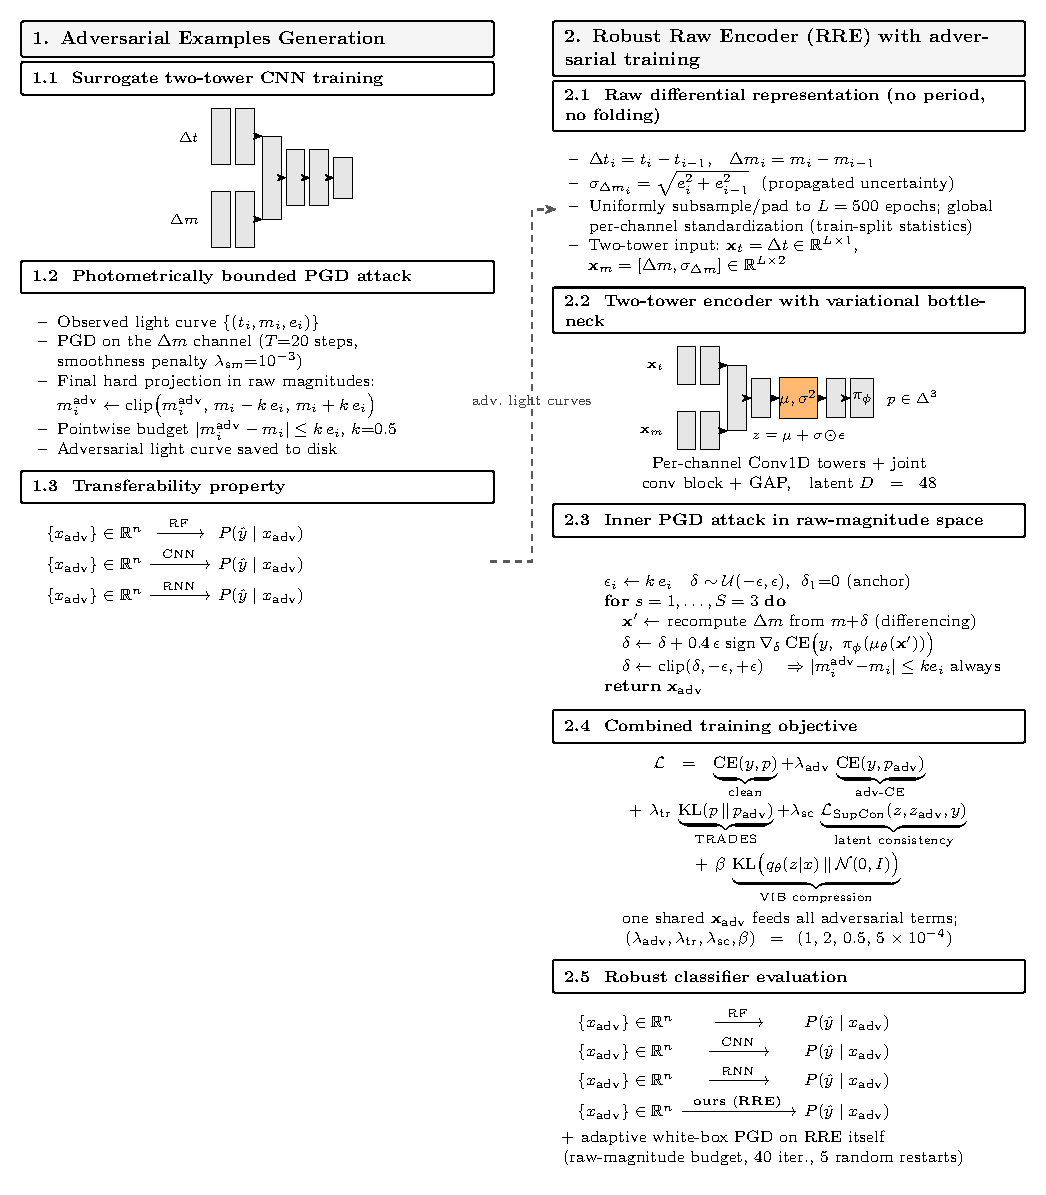
\includegraphics[width=\textwidth]{pipeline_overview.pdf}
  % Fuente: prueba/method_diagram_raw.tex (TikZ; recompilar con pdflatex).
  % Reemplaza al antiguo graphical_abstract.pdf (texto con kerning roto y
  % pipeline de fase obsoleto).
  \caption{Overview of the two-stage framework.
  \textbf{Stage~1 (left): photometry-constrained adversarial generation.}
  A surrogate two-tower CNN is trained on the differential representation
  $(\Delta t, \Delta m)$ of each light curve. Adversarial examples are crafted
  with a $T{=}20$-step PGD attack that perturbs only the magnitudes, under the
  per-point photometric budget $|m_i^{\mathrm{adv}}-m_i|\le k\,e_i$ with
  $k{=}0.5$; the resulting curves are transferred to the RF, CNN and RNN
  baselines.
  \textbf{Stage~2 (centre and right): Robust Raw Encoder (RRE).}
  The encoder ingests the raw differential representation
  $(\Delta t, \Delta m, \sigma_{\Delta m})$ directly. Two 1D-convolutional towers process the time and
  magnitude channels; their features are concatenated and compressed through a VIB, with the deterministic mean $\mu$
  used at inference. An inner PGD loop perturbs the raw magnitudes within the
  pointwise budget $|\delta_i|\le k\,e_i$ ($k{=}0.5$, $3$ steps, magnitude
  displacement clipped at every iteration) and recomputes $\Delta m$ by
  differencing, so that clean and on-the-fly adversarial views pass through
  the same encoder during training.
  A classifier head and an $\ell_2$-normalized projection head (for supervised
  contrastive learning) feed the full training objective
  $\mathcal{L}=\mathcal{L}_{\mathrm{CE}}(\mathrm{clean})
  +\lambda_{\mathrm{adv}}\mathcal{L}_{\mathrm{CE}}(\mathrm{adv})
  +\lambda_{\mathrm{tr}}\mathcal{L}_{\mathrm{TRADES}}
  +\lambda_{\mathrm{sc}}\mathcal{L}_{\mathrm{SupCon}}
  +\beta\,\mathcal{L}_{\mathrm{VIB}}$
  ($\lambda_{\mathrm{adv}}{=}1.0$, $\lambda_{\mathrm{tr}}{=}2.0$,
  $\lambda_{\mathrm{sc}}{=}0.5$, $\beta{=}5\times10^{-4}$). The trained model is
  evaluated under the same transferred attacks as the baselines.}
  \label{fig:pipeline}
\end{figure*}

\subsection{Latent-space stability under perturbation}
\label{app:latent}
\label{sec:latent_stability}

The accuracy figures of Sections~\ref{sec:l5_robustness}--\ref{sec:per_class}
show that the predicted class of the RRE classifier is essentially
unchanged by the adversarial attack, but they do not by themselves explain
how this stability arises inside the model. In this subsection we examine
the internal representation of clean and adversarial light curves to
identify the mechanism by which the RRE produces stable predictions.

We compare the learned latent space of the full RRE with that of its
V1 ablation (Section~\ref{sec:ablation}), trained on the same raw
two-tower $(\Delta t, \Delta m, \sigma)$ representation and the same
OGLE-III training split with clean cross-entropy only and no adversarial
component. The two encoders share the same Conv1D backbone, the same
latent dimensionality, and the same optimization protocol; they differ
solely in the training objective, so any difference between the two latent
spaces is attributable to the adversarial and regularization terms of the
RRE loss rather than to the architecture.

Figure~\ref{fig:latent_comparison_l1_vs_l5_raw} shows kernel-density
estimates of the first three latent means ($\mu_1, \mu_2, \mu_3$) of the
two encoders, for a representative class (LPV) of OGLE-III, separating the
clean test light curves (blue) from their adversarial counterparts
(orange). Panels (a)--(c) correspond to the V1 ablation and panels
(d)--(f) to the full RRE.

For the V1 ablation (left column), the clean and adversarial distributions
are visibly shifted along the latent axes: although the perturbation moves
every observation by at most $0.5\,e_i$ in magnitude, an encoder trained
without any adversarial objective maps the perturbed input to a measurably
different region of the latent space. Averaged over all $48$ latent
dimensions, the clean-to-adversarial displacement of the per-dimension
mean is $0.51\,\sigma$ for V1, with a two-sample Kolmogorov--Smirnov
statistic of $0.28$ between the clean and adversarial marginals,
confirming that the shift seen in panels (a)--(c) is representative of the
full latent space. This is the latent-space footprint of the adversarial
perturbation that drives the misclassification of the baseline classifiers
in Section~\ref{sec:attack_effectiveness}.

For the full RRE (right column), the clean and adversarial distributions
are essentially superimposed in all three latent dimensions, and the
all-dimension shift drops to $0.21\,\sigma$ (KS statistic $0.10$), less
than half that of the V1 ablation. The supervised
contrastive component $\mathcal{L}_{\mathrm{SupCon}}$ of the V5 loss
(Section~\ref{sec:loss}) explicitly forces clean and adversarial views of
the same light curve to be mapped to nearby points in latent space, while
the VIB $\mathcal{L}_{\mathrm{VIB}}$
compresses the representation enough to absorb the non-informative
variability introduced by the perturbation. The resulting latent space is
intrinsically insensitive to perturbations within the photometric-error
budget, which is the structural reason behind the near-zero adversarial
drop reported in Tables~\ref{tab:main_multisurvey}
and~\ref{tab:per_class_l5_multi}.

{\setlength{\textfloatsep}{8pt plus 2pt minus 4pt}
\begin{figure}[htbp]
\centering
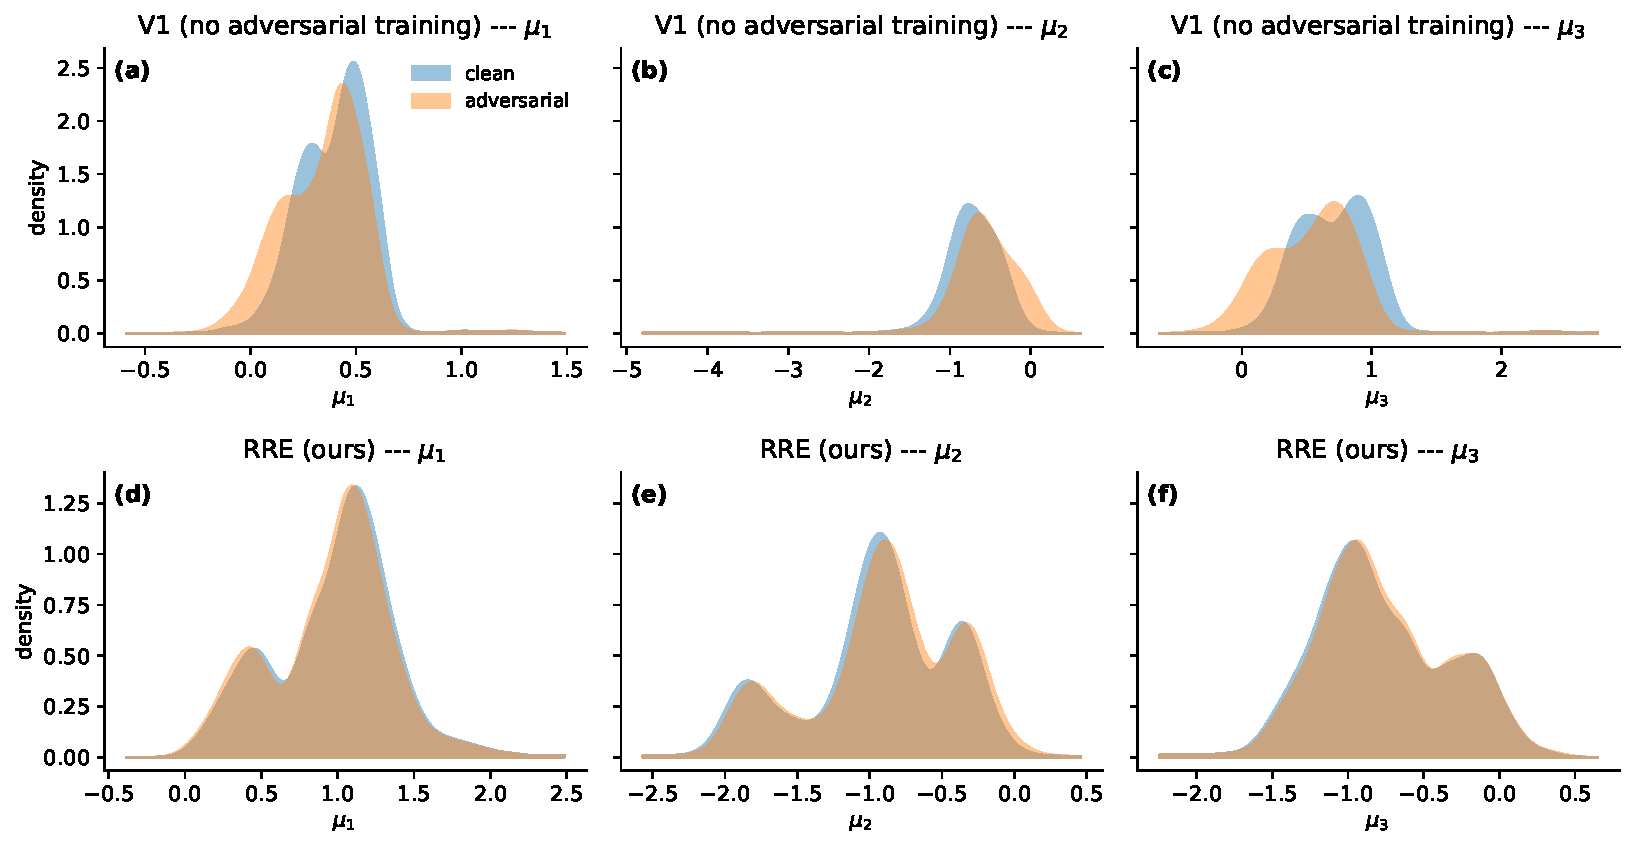
\includegraphics[width=\columnwidth]{latent_comparison_l1_vs_l5_raw.pdf}
\caption{Kernel-density estimates of the first three latent means
($\mu_1, \mu_2, \mu_3$) for OGLE-III LPV light curves, clean (blue) and
adversarial (orange). Panels (a)--(c) (left column) correspond to the V1 ablation
(clean cross-entropy only, no adversarial component); panels (d)--(f)
(right column) correspond to the proposed full RRE classifier. Both encoders share the
same raw two-tower $(\Delta t, \Delta m, \sigma)$ architecture and differ
solely in the training objective. The clean and adversarial distributions
are visibly shifted in the V1 latent space and superimposed in the RRE
latent space, illustrating the role of the adversarial, supervised
contrastive, and information-bottleneck components of the full V5
objective.}
\label{fig:latent_comparison_l1_vs_l5_raw}
\end{figure}

\begin{figure}[htbp]
\centering
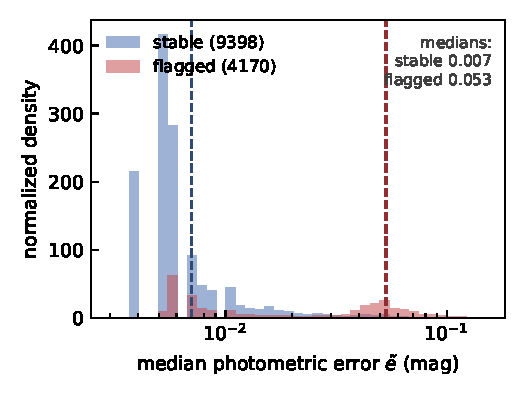
\includegraphics[width=0.78\columnwidth]{flag_quality.pdf}
\caption{Distribution of the median reported photometric error
$\tilde{e}$ for OGLE-III sources whose CNN prediction is flipped by the
transferred attack (flagged) versus those that are stable. Flagged
sources are systematically noisier (median $0.053$ vs.\ $0.007$~mag;
Mann--Whitney $p \ll 10^{-100}$), showing that the robustness flag of
Section~\ref{sec:discussion} tracks genuine data quality. Dashed lines
mark the two medians; the horizontal axis is logarithmic.}
\label{fig:flag_quality}
\end{figure}
} % end \setlength{\textfloatsep}



\begin{table}[htbp]\centering
\caption{Per-source robustness flag: fraction of test predictions that
change under the transferred attack ($k=0.5$), i.e.\ the sources that the
audit would route to follow-up. Absolute counts in parentheses. The
margin-resolved view is given in Fig.~\ref{fig:flip_rate}.}
% Fuente: outputs/metrics/flip_rate_audit.csv
% (python3.12 -m src.experiments.flip_rate_audit)
\label{tab:flip_rates}
\small
\begin{tabular}{lcc}
\toprule
Survey & CNN & RRE (ours) \\
\midrule
OGLE-III          & $30.7\%$ $(4170/13568)$ & $0.4\%$ $(56/13568)$ \\
\textit{Gaia} DR2 & $1.8\%$ $(209/11483)$   & $0.5\%$ $(63/11483)$ \\
WISE              & $9.8\%$ $(853/8704)$    & $0.5\%$ $(45/8704)$  \\
\bottomrule
\end{tabular}
\end{table}

\FloatBarrier
% --------------------------------------------------------------------------

\section{Additional robustness controls}
\label{app:controls}

This appendix collects the control experiments summarized in
Sect.~\ref{sec:ablation}: the random-noise-augmentation baseline, the
component controls without adversarial cross-entropy, and the VIB-only
$\beta$-sweep.



\subsection{Component controls without adversarial cross-entropy}
\label{app:component_controls}

To separate adversarial cross-entropy from the other terms, we trained
controls that activate each family of terms without AdvCE
(Table~\ref{tab:component_controls}).

\begin{table}[htbp]
\centering
\caption{Component controls on OGLE-III under the transferred CNN-targeted
attack ($k=0.5$). These runs use the same raw two-tower architecture and
training split as Table~\ref{tab:ablation_robust}, but isolate whether a
loss family can produce robustness without adversarial cross-entropy. Drop
is $\mathrm{acc}_{\mathrm{c}}-\mathrm{acc}_{\mathrm{a}}$ in percentage
points, so smaller is better.}
% Source CSV: outputs/metrics/ogle/component_attribution_summary.csv
\label{tab:component_controls}
\small
\setlength{\tabcolsep}{3pt}
\resizebox{\columnwidth}{!}{%
\begin{tabular}{llrrr}
\toprule
Variant & Active components & $\mathrm{acc}_{\mathrm{c}}$ & $\mathrm{acc}_{\mathrm{a}}$ & drop \\
\midrule
V2 & CE + AdvCE & 0.984 & 0.979 & 0.45 \\
TRADES-only & CE + TRADES & 0.983 & 0.979 & 0.37 \\
Aux-no-AdvCE & CE + TRADES + SupCon + VIB & 0.982 & 0.977 & 0.49 \\
SupCon-only & CE + SupCon & 0.988 & 0.943 & 4.44 \\
VIB-only & CE + VIB & 0.985 & 0.905 & 8.01 \\
\bottomrule
\end{tabular}
}
\end{table}

The controls refine the interpretation of the V5 objective. Clean
cross-entropy plus TRADES alone reaches $0.983$ clean and $0.979$
adversarial accuracy, indistinguishable from V2 under the transferred
attack; the combination of TRADES, SupCon and VIB without adversarial
cross-entropy remains similarly robust ($0.982 \to 0.977$). By contrast,
SupCon alone is only partially robust ($0.988 \to 0.943$), and VIB alone
is not robust (Sect.~\ref{app:vib_only}). The pairwise error-overlap
analysis also does
not support a simple interpretation in which each term protects a separate
observational regime: relative to V2, V4 rescues 78 of the 280 V2
adversarial errors while introducing 46 new ones, whereas V5 and
TRADES-only exchange nearly equal numbers of objects. The empirical
message of the ablation is that the raw representation becomes robust when
clean and photometrically bounded adversarial views are explicitly coupled
during training; the full V5 objective keeps this robust solution while
also imposing the representation-level structure that motivates the latent
analysis.

\subsection{The bottleneck alone provides no robustness}
\label{app:vib_only}
% Source CSV: outputs/metrics/ogle/vib_only_beta_sweep.csv
Because the variational bottleneck has occasionally been proposed as an
intrinsically robustness-inducing mechanism \citep{alemi2017deep}, we also
trained the complementary configuration: clean cross-entropy plus VIB only,
with \emph{no} adversarial component, sweeping
$\beta \in \{5\times10^{-4}, 10^{-3}, 10^{-2}, 10^{-1}\}$. All four models
retain high clean accuracy ($0.985$--$0.987$) but lose $8.0$--$9.4$~pp
under the same transferred attack --- a drop that \emph{grows} with the
compression strength --- and a stronger bottleneck ($\beta=1$) collapses to
the majority class. Information compression alone therefore does not
confer robustness within the photometric threat model: the explicit
clean--adversarial coupling provided by AdvCE or TRADES is the operative
ingredient, and VIB earns its place only as a latent-space regularizer on
top of that coupling. This finding independently corroborates
\citet{korshunova2021closer}, who showed on image benchmarks that
information-bottleneck models alone are not a strong defense and that
earlier positive results were affected by gradient obfuscation --- a
concern our adaptive evaluation (Sect.~\ref{sec:adaptive_attack})
addresses by attacking through the deterministic encoder mean.

\begin{figure*}[htbp]
\centering
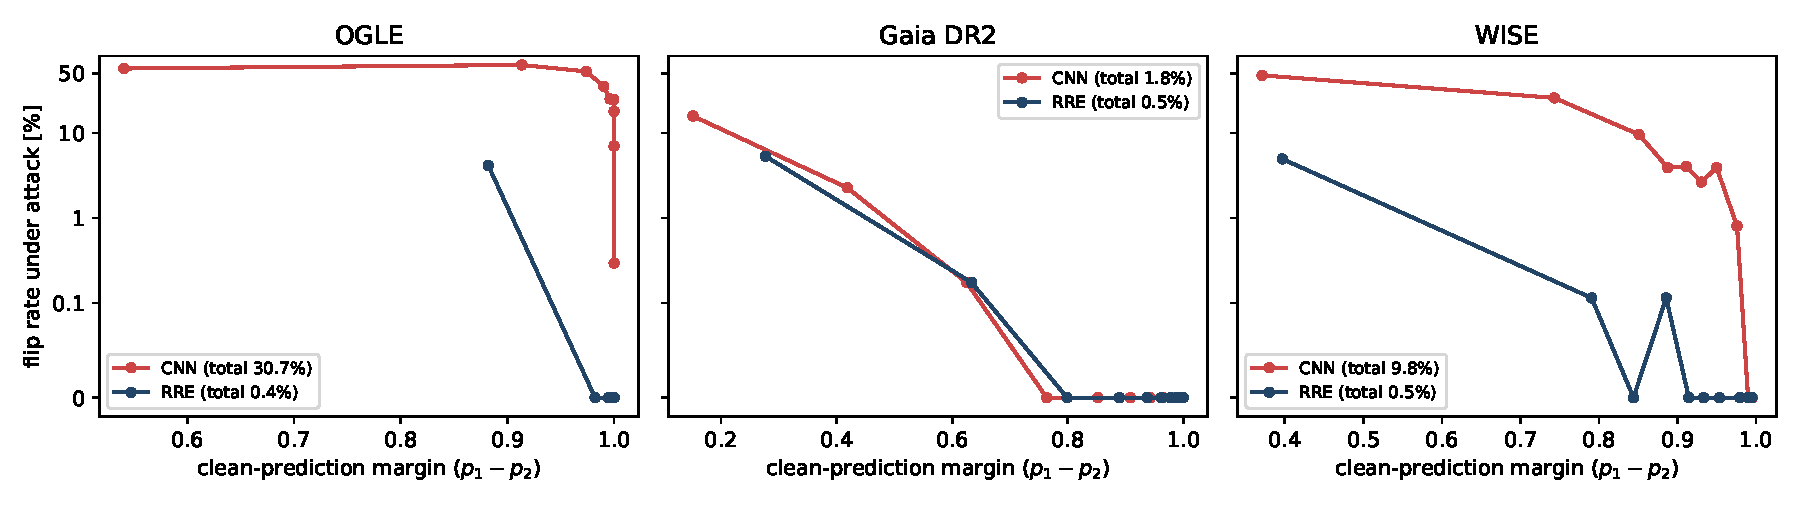
\includegraphics[width=0.68\textwidth]{flip_rate_vs_margin.pdf}
% Fuente: python3.12 -m src.experiments.flip_rate_audit
\caption{The per-source robustness flag in practice (discussed in
Sect.~\ref{sec:discussion}): fraction of test
predictions that change under the transferred attack ($k=0.5$) as a
function of the clean-prediction margin $p_1 - p_2$, in margin deciles
(symlog vertical scale; legend gives the survey-wide flip fraction of each
model). Deciles are computed per model and each point is drawn at the
median margin of its decile, so the horizontal extent of a curve reflects
that model's confidence distribution: the RRE curve on OGLE-III begins
near margin $0.9$ because even its lowest-confidence decile is that
confident. For the defended RRE (blue), prediction changes are rare and
concentrate at low margin, so margin plus the adversarial flip flag
identifies the small subset of sources (${\sim}0.5\%$) whose
classifications warrant follow-up. For the undefended CNN (red), flips
persist at margins close to $1$ on OGLE-III and WISE: high reported
confidence does not certify stability within the photometric error bars.}
\label{fig:flip_rate}
\end{figure*}

\section{Gradient-free, margin-based, and attack-potency checks: protocols}
\label{app:sanity_checks}

\begin{table}[htbp]\centering
\caption{Adaptive white-box PGD evaluated on RRE's \emph{own} gradient ($T=40$ steps, per-point step $0.1\,\epsilon_i$, $5$ random restarts, raw-magnitude displacement bounded by $k\,e_i$ with $k=0.5$), following the adaptive-evaluation recommendations of \citet{carlini2019evaluating}. Even under a first-order attack that directly follows the defended model's gradient, the accuracy drop does not exceed one percentage point. This is evidence against simple gradient masking, not a certificate of robustness. All values are percentages.}
\label{tab:adaptive_pgd}
\small
\begin{tabular}{lccc}
\toprule
Survey & Clean & Adaptive PGD & Drop (pp)\\
\midrule
OGLE-III & 98.3 & 97.3 & $-1.0$\\
\textit{Gaia} DR2 & 91.1 & 90.4 & $-0.7$\\
WISE & 93.2 & 92.5 & $-0.7$\\
\bottomrule
\end{tabular}
\end{table}
% Fuentes: outputs/metrics/ogle/l5_raw_square_attack_k0.50.csv,
% adaptive_pgd_l5_raw_k5.00.csv, adaptive_pgd_l5_raw_k20.00.csv,
% adaptive_pgd_dlr_k0.50_T40.csv, adaptive_pgd_dlr_k0.50_T100.csv.

Following the evaluation checklist of \citet{carlini2019evaluating}, we
complement the adaptive PGD with three further checks on OGLE-III.

First, a \emph{gradient-free} attack: because the encoder contains a
stochastic bottleneck --- precisely the component that
\citet{korshunova2021closer} showed can obfuscate gradients --- we ran
the same score-based Square-style search used against the RF
(Sect.~\ref{sec:attack_effectiveness}), perturbing the raw magnitudes of
a stratified subsample of $800$ test curves within the $k=0.5$ budget and
querying the RRE class probabilities at every step. After $1{,}000$
iterations the accuracy declines only from $0.976$ to $0.974$
($-0.25$~pp), against $-0.37$~pp for the white-box adaptive PGD run on
the \emph{same} $800$-curve subsample ($0.976 \to 0.973$; the full-test
white-box drop is $-1.0$~pp): the gradient-based attack is consistently
stronger than the gradient-free one, which is the expected signature of a
model whose gradients are informative rather than masked
\citep{athalye2018obfuscated}.

Second, a \emph{margin-based} objective: we replaced the cross-entropy of
the adaptive attack with the untargeted DLR loss of APGD
\citep{croce2020reliable}, computed exactly from the classifier
log-probabilities (softmax shift-invariance makes logit differences equal
to log-probability differences). At $T=40$ with five restarts the DLR
attack reaches $0.973$, identical to the cross-entropy attack, and
extending to $T=100$ changes nothing ($0.973$): the attack is converged,
and the margin objective finds no additional adversarial examples.

Third, an \emph{attack-potency} diagnostic outside the threat model:
rerunning the adaptive PGD with the budget inflated to $k=5$ and $k=20$
--- physically inadmissible displacements of five and twenty reported
uncertainties per point --- collapses the accuracy to $0.135$ (below the
four-class random-guess level) and $0.007$, respectively. The same attack
configuration that annihilates the model when given room is therefore the
one that fails to move it inside the photometric error bars, confirming
that the robustness at admissible budgets reflects the threat model, not
an under-converged attack.



\section{Survey details}
\label{app:surveys}

This appendix documents the composition of the three catalogs used in
this work. Table~\ref{tab:survey_classes} lists the native variability
classes of each survey together with the number of sources available
before any selection, as compiled by \citet{becker2020scalable}. The
native labels differ between surveys --- OGLE-III uses aggregate
morphological classes, \textit{Gaia} DR2 reports the pulsation-mode
labels of its variability pipeline, and the WISE catalog inherits the
OGLE-III nomenclature --- so Table~\ref{tab:class_balance} shows how they
are grouped into the four working classes used throughout the paper, and
Table~\ref{tab:counts} gives the resulting per-class train/test counts
after the per-class cap and the stratified split. Together they make
explicit the class imbalance that drives the WISE per-class results of
Appendix~\ref{app:perclass}: the CEP and DSCT populations there are one
to two orders of magnitude smaller than RRLYR and LPV.


\begin{table}[htbp]\centering
\caption{Native catalog labels of each survey, grouped into the working
classes of this paper: RR~Lyrae (RRL), Cepheids (CEP), long-period
variables (LPV), $\delta$~Scuti/SX~Phoenicis (DSCT), and eclipsing binaries
(ECL). Numbers are sources available before any selection
\citep{becker2020scalable}; bold rows give the class totals. Subtype labels
use a common notation across surveys. OGLE-III provides only aggregate
classes (its ECL class aggregates EC, ESD, and ED; LPV aggregates Mira,
SRV, and OSARG; RRL aggregates RRab and RRc), so its subtype counts are
not listed. A dash means that the class or subtype is absent from that
catalog.}
\label{tab:survey_classes}
\footnotesize
\setlength{\tabcolsep}{3.5pt}
\begin{tabular}{@{}llrrr@{}}
\toprule
Class & Subtype & OGLE-III & \textit{Gaia} DR2 & WISE\\
\midrule
\textbf{RRL} & & \textbf{33{,}933} & \textbf{195{,}515} & \textbf{20{,}488}\\
 & RRab & & 162{,}244 & 16{,}412\\
 & RRc & & 32{,}331 & 3{,}831\\
 & RRd & & 834 & 241\\
 & anomalous RRd & & 106 & 4\\
\midrule
\textbf{CEP} & & \textbf{7{,}836} & \textbf{8{,}542} & \textbf{2{,}419}\\
 & classical & & 6{,}488 & 1{,}884\\
 & type~II & & 1{,}740 & 482\\
 & anomalous & & 314 & 53\\
\midrule
\textbf{LPV} & & \textbf{275{,}857} & \textbf{150{,}215} & \textbf{63{,}891}\\
 & Mira + SRV & & 150{,}215$^{a}$ & 10{,}001\\
 & OSARG & & -- & 53{,}890\\
\midrule
\textbf{DSCT} & & 2{,}822$^{b}$ & \textbf{8{,}870} & \textbf{1{,}098}\\
\textbf{ECL} & & \textbf{37{,}840} & -- & --\\
\midrule
Not used & non-variable & 34{,}815 & -- & 32{,}795\\
 & NC, ELL, C$^{c}$ & -- & -- & 2{,}548\\
\midrule
\emph{Total} & & 393{,}103 & 363{,}142 & 123{,}239\\
\bottomrule
\end{tabular}
\tablefoot{
$^{a}$~\textit{Gaia} DR2 reports Miras and semiregulars as a single class
(MIRA\_SR); in WISE they are $1{,}396$ Miras and $8{,}605$ SRVs.
$^{b}$~Present in the OGLE-III catalog but not used: the OGLE-III
experiment adopts its four most populated classes.
$^{c}$~Non-classified, ellipsoidal, and other WISE groups.}
\end{table}

\begin{table}[htbp]\centering
\caption{Final per-class train/test counts and epoch distribution, from a stratified 70/10/20 split (seed~42) after capping each class at $20{,}000$ objects. Train aggregates train$+$validation ($70\%+10\%$); minority-class counts are exact to within rounding ($\le4$). Epochs are median [IQR] over the test set; $L=500$ is the imposed maximum length (Sect.~\ref{sec:input_rep}), not the native cadence.}
\label{tab:counts}
\footnotesize
\begin{tabular}{llrrr}
\toprule
Survey & Class & Train & Test & Epochs\\
\midrule
\multirow{5}{*}{OGLE-III}
 & ECL & 16,000 & 4,000 & 500\\
 & RRL & 16,000 & 4,000 & 500\\
 & CEP & 6,268 & 1,568 & 500\\
 & LPV & 16,000 & 4,000 & 500\\
 & \emph{All} & 54,268 & 13,568 & 500 [436,500]\\
\midrule
\multirow{5}{*}{\textit{Gaia} DR2}
 & RRL & 16,000 & 4,000 & 20\\
 & LPV & 16,000 & 4,000 & 23\\
 & CEP & 6,833 & 1,709 & 26\\
 & DSCT & 7,096 & 1,774 & 20\\
 & \emph{All} & 45,929 & 11,483 & 23 [15,30]\\
\midrule
\multirow{5}{*}{WISE}
 & RRL & 16,000 & 4,000 & 29\\
 & LPV & 16,000 & 4,000 & 82\\
 & CEP & 1,935 & 484 & 49\\
 & DSCT & 878 & 220 & 27\\
 & \emph{All} & 34,813 & 8,704 & 48 [28,84]\\
\bottomrule
\end{tabular}
\end{table}

\begin{table}[htbp]
\centering
\caption{Per-survey class counts after grouping the native catalog labels of Table~\ref{tab:survey_classes} into the four working classes of this paper, before the per-class cap of $20{,}000$ objects and the train--test split (Table~\ref{tab:counts}). Per-class numbers explain the WISE failure mode on CEP and DSCT discussed in Appendix~\ref{sec:per_class}.}
\label{tab:class_balance}
\small
\begin{tabular}{lrrrrr}
\toprule
Survey & RRLYR & ECL & LPV & CEP & DSCT \\
\midrule
OGLE-III & 33{,}933 & 37{,}840 & 275{,}857 & 7{,}836 & -- \\
\textit{Gaia} DR2 & 195{,}515 & -- & 150{,}215 & 8{,}542 & 8{,}870 \\
WISE & 20{,}488 & -- & 63{,}891 & 2{,}419 & 1{,}098 \\
\bottomrule
\end{tabular}
\end{table}


% - join the .bib files when you upload your source files
%%%%%%%%%%%%%%%%%%%%%%%%%%%%%%%%%%%%%%%%%%%%%%%%%%%%%%%%%%%%%%


% %%%%%%%%%%%%%%%%%%%%%%%%%%%%%%%%%%%%%%%%%%%%%%%%%%%%%%%%%%%%%%
% Example below of non-structurated natbib references  
% To use the v8.3 macros with this form of composition of bibliography,
% the option "bibyear" should be added to the command line
% "\documentclass[bibyear]{aa}".
% %%%%%%%%%%%%%%%%%%%%%%%%%%%%%%%%%%%%%%%%%%%%%%%%%%%%%%%%%%%%%%


%%%%%%%%%%%%%%%%%%%%%%%%%%%%%%%%%%%%%%%%%%%%%%%%%%%%%%%%%%%%%%%
% Appendices must be placed after   \end{thebibliography}
% They will be placed automatically on a new page.
%%%%%%%%%%%%%%%%%%%%%%%%%%%%%%%%%%%%%%%%%%%%%%%%%%%%%%%%%%%%%%%



\FloatBarrier %\usepackage{placeins}

\section{Baseline configurations}
\label{app:baselines}

All baselines share the split, seed, and preprocessing of
Section~\ref{results_setup}; the trained checkpoints and training scripts
are part of the released repository (Section~\ref{sec:implementation}).

\paragraph{Random Forest (RF-FATS16).}
he RF operates on $16$ hand-crafted, period-independent features computed
from the raw magnitudes and reported errors of each curve
(Table~\ref{tab:fats16}); they follow the spirit of the FATS library
\citep{nun2015fats} but are recomputed by our pipeline, which is what
allows the black-box attack of Sect.~\ref{sec:attack_effectiveness} to
re-evaluate them at every query. The classifier is a
\texttt{scikit-learn} \texttt{RandomForestClassifier} with $300$ trees and
maximum depth $25$; all other hyperparameters are left at their
\texttt{scikit-learn} defaults ($\sqrt{d}$ features per split, minimum leaf
size $1$), and the random seed is fixed to $42$ for reproducibility. These
values were set a priori rather than tuned by grid search: random-forest
accuracy is known to be insensitive to them once a few hundred trees are
used \citep{breiman2001random,hastie2009elements}, and the resulting
classifier is a strong baseline ($96.9\%$ clean accuracy on OGLE-III),
so its vulnerability is not an artifact of under-fitting.

\begin{table}[htbp]\centering
\caption{The 16 features of the RF baseline, computed from the raw
magnitudes $m_i$ and reported errors $e_i$ (no period information).}
\label{tab:fats16}
\small
\setlength{\tabcolsep}{4pt}
\begin{tabular}{ll}
\toprule
Feature & Definition \\
\midrule
\texttt{n\_obs} & number of observations \\
\texttt{median} & median magnitude \\
\texttt{weighted\_mean} & inverse-variance weighted mean \\
\texttt{weighted\_std} & inverse-variance weighted std.\ dev. \\
\texttt{amplitude} & $(\max m - \min m)/2$ \\
\texttt{iqr} & interquartile range \\
\texttt{mad} & median absolute deviation \\
\texttt{skew}, \texttt{kurtosis} & standardized third/fourth moments \\
\texttt{stetson\_k} & Stetson $K$ robust shape statistic \\
\texttt{beyond1std} & fraction of points beyond $1\sigma$ of mean \\
\texttt{slope\_p10}, \texttt{slope\_p90} & sorted-magnitude tail slopes \\
\texttt{eta} & von Neumann ratio $\eta$ \\
\texttt{mean\_err}, \texttt{median\_err} & mean / median reported error \\
\bottomrule
\end{tabular}
\end{table}

\paragraph{Surrogate CNN.}
The two-tower CNN of Sect.~\ref{cnn_classifier} applies two
weight-shared convolutional blocks to each channel --- Conv1D($32$,
kernel $15$, stride $2$, ReLU) followed by Conv1D($16$, kernel $11$,
stride $2$, ReLU) --- concatenates the two feature maps, and classifies
through Flatten $\to$ Dropout($0.5$) $\to$ Dense($64$, tanh) $\to$
Dropout($0.5$) $\to$ Softmax($4$), for $2.6\times10^{5}$ trainable
parameters. It is trained with Adam (learning rate $10^{-3}$),
categorical cross-entropy, batch size $256$, for up to $50$ epochs with
early stopping on the validation loss (patience $5$, best weights
restored).

\paragraph{Recurrent baseline (GRU).}
The RNN concatenates the $(\Delta t, \Delta m)$ channels into a
$(L, 2)$ sequence processed by a single GRU layer of $64$ units followed
by a softmax layer. It is trained with Adam ($10^{-3}$), categorical
cross-entropy, batch size $256$, early stopping on the validation
accuracy (patience $4$) and learning-rate halving on plateau
(patience $2$).

\end{document}
